% !TEX root = Mein Credo.tex
\part{Überprüfung der Bibel auf Ihre Glaubwürdigkeit}
\chapter{Die Bibel als Hauptkern des Christlichen Glaubens}
Ein umstrittener Grund des christlichen Glaubens ist, worauf sie sich beruft: Die heilige Schrift, auch Bibel genannt. Sie ist das Fundament der Kirche. Um die Wahrhaftigkeit dieses Schriftstückes feststellen zu können, muss sie auf ihre Stichhaltigkeit geprüft werden. Nur eine stichhaltige Quelle kann als Beweis angesehen werden, vor allem wenn der Glaube aus einer Zeit entspringt, wo andere Völker den polytheistischen Kult verehrten. In einer Zeit, in welcher Wissenschaft das war, was ein absolutistischer Herrscher von sich gab. In einer Zeit voller unbegründeter Irrlehren und falschen Ansichten. Zudem besteht das Risiko von Zudichtungen, die unvermeidlich über die Jahrhunderte bis zur Kanonisierung ihren Weg in die Schriften gefunden haben könnten.
\\~\\
Um seinen Glauben beweisen zu können, muss man erstmal die Bibel beweisen bzw.\ sie auf ihre Glaubwürdigkeit prüfen. Aus Sicht eines Glaubenden hat Gott die Quellenträger, die Verfasser und die Kirchenväter geleitet, sodass die Bibel im Zusammenhang als komplett wahr zu betrachten ist. Aus theologischer Sicht ist die Bibel stichhaltig oder treffender gesagt: Sie ist das Wort Gottes. Jedoch wird auch versucht, die Bibel wissenschaftlich und ohne Berücksichtigung der Theologie auf ihre Glaubwürdigkeit zu prüfen.

\section{Kriterien für die Überprüfung}
Primäres Ziel ist die Überprüfung der Quellen auf ihre Glaubwürdigkeit. Dazu werden die Quellen der einzelnen Schriften ausfindig gemacht und auf ihre Glaubwürdigkeit und ihre göttliche Inspiration überprüft. Dafür werden die Autoren identifiziert oder auf einen Personenkreis oder Gruppe eingegrenzt.
Da die Entstehung der Bibel heutzutage immer noch umstritten ist, sind alle Ergebnisse als Theorien und nicht als feststehende Sachverhalte zu verstehen.
\\~\\
Wichtig zu wissen ist, dass diese Kriterien von mir aus rein persönlichen Gründen gewählt wurden und nicht mit wissenschaftlichen Kriterien übereinstimmen müssen. Trotzdem sollten sich diese Kriterien mit den gängigen wissenschaftlichen Methoden decken.

\chapter{Untersuchung der Bibel anhand überlieferter Manuskripte}
Es werden alle überlieferten Manuskripte, egal aus welcher Hand, ausgewertet. Von diesen sind über 5600 griechische, 10.000 Lateinische und 5.000--10.000 andere vorhanden. Bei Gaius Julius Cäsar waren es 10.  Aus diesen gehen eine Anzahl von 300.000--400.000 Lesearten des Neuen Testaments hervor. Davon werden irrelevante ausgefiltert, welche zum Beispiel aufgrund von stilistischen und grammatikalische Unterschiede raus fallen. Schlussendlich gibt es 400 Lesearten, die Zweifel an der Zuverlässigkeit der Bibel wecken könnten. Davon sind aber nur 50 von größerer Wichtigkeit und es handelt sich bei diesen auch nicht um essentielle Kernbotschaften der christlichen Lehre. Für antike Verhältnisse eine verschwindend geringe Anzahl, welche es in diesen Dimensionen sonst nicht gibt. Rein rechnerisch ist der Text zu 98,33\% rein. Demnach wurde das neue Testament ohne Unterschiede überliefert. Bibliographisch gesehen ist das Neue Testament bibliographisch zuverlässig.
\\
Zusätzlich zu den ca. 20.000 Manusskripten kommen dann noch ca. 1 Million Zitierungen der Kirchenväter hinzu, mit dieser man das neue Testament (fast) komplett rekonstruieren könnte. Eine gängiges Gegenargument hierbei ist, dass 96\% der Manusskripte aus der Zeit ab den 8. Jahrhundert stammen. Dieser Anteil der Manusskripte verursachen aber nur 2\% der hinzugekommenen Materialen.
\\~\\
Das Alte Testament kann auch anhand der Manuskripte hinsichtlich seiner historischen Verlässlichkeit geprüft werden. Dies ist mit den Talmundisten und Masoreten zu bewerkstelligen. Diese schreiben das alte Testament mit größter Sorgfalt ab. Strenge, festgelegte Regeln sollten fehlerfreie Kopien des alten Testaments bzw.\ der Thora gewährleisten. So zählten sie z.B. die Worte, die Seiten, das mittlere Wort einer Schrift und vieles mehr. Mithilfe dieser Methoden wollten sie sicherstellen, dass die Schriften komplett richtig abgeschrieben werden. Die kleinste Abweichung machte die Schrift unbrauchbar und sie wurde vernichtet. Ist der Text abgefasst worden und das Manuskript zu sehr gealtert, dann wurde diese auch entsorgt. Der Grund für die (vergleichsweise kleine) Anzahl der überlieferten Manuskripte ist der, dass alle fehlerhaften Schriften unverzüglich entsorgt wurden. Diese Arbeitsmethoden der Juden und später der Christen im Mittelalter, die die Methoden der Masoreten kopierten, stellen die historische Verlässlichkeit des Alten Testaments fest.
\\~\\
Beide Theorien werden mit archäologischen Funden gestützt wie z.B. den Fund der Schriftrollen der Qumran-Höhlen. Diese beweisen, dass die Bibel, wie wir sie heute kennen, mit der damaligen Fassungen nahezu komplett übereinstimmen. Die Bibel ist also bibliographisch Zuverlässig. Oder trivial gesagt: Die Bibel wurde über die Zeitspanne von 3000--4000 Jahren nicht schwerwiegend verfälscht! Man darf sich natürlich nicht der Blendung hingeben, dass alles garantiert richtig überliefert ist -am Ende handelt es sich immernoch um ein 2000 Jahre altes Poesiewerk-, aber für so ein Werk kann man schon ein sehr hohes Vertrauen in seinen Inhalt mitbringen. Das die Schriften von Gott inspiriert sein könnten, wird im Folgendem  bei jeden einzelnen Autor überprüft, auch wenn dies nicht wissenschaftlich bewiesen oder widerlegt werden kann. 

\chapter{Das Alte Testament}
Das Alte Testament ist (wie das Neue Testament) eine Sammlung vieler Schriften mit noch mehr Autoren und vermutlich Redakteuren. Eine Überprüfung jeder einzelnen Schrift ist unumgänglich. Da für die Zeit bis 1200 v. Chr.\ weder archäologische noch historische Entdeckungen gemacht wurden, kann für diese Zeit keine Aussagen zu den Autoren und die Glaubwürdigkeit der Schriften gemacht werden. Diese Berichte können einzig und allein als Mythen deklariert werden. Eine Untersuchung ist erst ab diesen Zeitpunkt sinnvoll. Dies ist die Zeit des König Davids.

\section{Pentateuch}
Lange Zeit wurde angenommen, dass die fünf Bücher Mose (Pentateuch) von Mose geschrieben wurden. Jedoch fand man heraus, dass es innerhalb der Schriften Dubletten gibt. Diese Dubletten unterschieden sich wesentlich. Es gibt verschiedene Schreibstile. So wird z.B. Gott als Jahwe und als Gott bezeichnet. Es gibt unterschiedliche Versionen der ein und derselben Geschichte.So unterscheidet sich zum Beispiel die Kalbsgeschichte, in welcher Aaron und das Volk Israel ein goldenes Kalb erschaffen und es anbeteten. Unter anderen darauf baut sich die neuere Urkundenhypothese auf. Diese behauptet, dass die fünf Bücher Mose von vier verschiedenen Autoren geschrieben und von einen Redakteur zusammengetragen wurden. Die Autoren werden als Quellenschichten (Jahwist-, Elohistschicht, den Priesterkodex und Deutoromium)  bezeichnet. Ihre Identität ist bis heute unbekannt und wird vermutlich für immer unbekannt bleiben.

\subsection*{Jahwist und Elohist}
Der Jahwist lebte vermutlich während der Zeit, in der Israel durch den König Rehabeam in Israel und Juda geteilt wurde. Es ist aus seinen Berichten zu entnehmen, dass er die Abspaltung Edoms noch miterlebt hat, jedoch zur Zerstörung Israels verstorben war, was seine Lebenszeit auf 848--722 v. Chr.\ eingrenzt. Der Jahwist gehörten dem Volk Juda an, woraus David und Salomo stammten.
\\~\\
Der Elohist hingegen lebte in Israel. Er war damit ein Feind Judas und so auch anderer Auffassungen als der Jahwist. Es ist aufgrund seiner Darstellung der biblischen Geschichten anzunehmen, dass der Elohist Verbindungen zu der levitischen Priesterschaft pflegte. Zusammen mit dieser Beziehung und der männlich-orientierten Erzählperspektive liegt die Vermutung nahe, dass der Elohist ein Mann war.
\\~\\
Um die verschiedene Versionen der ein und derselben Geschichten, welche zum Teil sich gegenseitig widersprachen, erklären zu können, muss man die Geschichte des Königreichs Israel betrachten. König David -eine der längsten währenden Königsdynastien überhaupt- vereinte die zwölf Stämme Israels erstmals zu einen großen Königreich mit ein und derselben Religion und Gott: Jahwe. Das Königreich überlebte die Streite über die Erbschaft bis zu König Salomo. König Rehabam wurde der neue König und wollte sich im Nordreich krönen wollen. Das Nordreich fragte, ob er die Politik seines Vaters fortführe, welcher das Nordreich benachteiligt hatte zugunsten von Juda. Er bejahte und so spaltete sich das Nordreich Israel ab und wählte Jerobeam zum neuen König. Das Reich war gespalten, aber der gemeinsame Glaube war noch da.
\\~\\
Die Reliquien befanden sich in Jerusalem, der Hauptstadt Judas. König Jerobeam konnte und wollte nicht riskieren, dass viele Bürger des Nordreiches regelmäßig nach Jerusalem pilgern und sich den judäischen Einfluss aussetzten. Also schuf Jerobeam neue religiöse Symbole, Feiertage, eine neue Priesterschaft und zwei neue religiöse Zentren: Beth-El und Dan. Da Politik und Religion zu der Zeit ein und dasselbe war, musste Jerobeam und bzw.\ der Elohist das Nordreich dies legitimieren. Der Elohist gehörte vermutlich zu den Priestern von Silo, sprich zu den Leviten, welche heimatlos und so sowohl im Nordreich als auch in Juda fremd waren. Er wählte das kleinere Übel und schrieb die Passagen so nieder, um wahrscheinlich im Nordreich eine Chance auf die Priesterschaft zu haben. Der Jahwist gehörte vermutlich Juda an und berichtete genauso wie der Elohist zum Vorteil seines Reiches.
\\~\\
Der Kern der Schriften blieb jedoch identisch. Entweder, weil die eine Fassung eine überarbeitete Fassung der anderen Fassung ist oder weil beide auf eine selbe Basis aufbauten. Nach der Zerstörung des Nordreiches durch die Assyrer flohen die Menschen nach Juda und führten vermutlich die Schrift des Elohisten mit sich. Die Integration war nicht schwer. Dieselbe Patriarchen, derselbe Gott, und dieselbe Sprache gab den Menschen eine gemeinsame Identität. Doch es gab zwei heilige Schriften. Zwar gab es einen gemeinsamen Kern, jedoch gab es bei der Charakterisierung von zentralen Personen und der Darstellungsweise von einigen Geschichten wie z.B. das goldene Kalb Diskrepanzen. Anstatt eine Schrift zu bevorzugen und die andere für nichtig zu erklären, ließ man beide vermutlich zu einer Schrift verschmelzen, um Konflikte zu vermeiden und die Stabilität des Landes zu gewährleisten. Eine neue heilige Schrift wurde geschaffen, eine Mixtur von den Jahwisten und den Elohisten.

\subsection*{Priesterschrift}
Die Priesterschrift bildet die größte Quellenschicht, größer als J, E und D zusammen. Lange Zeit wurde angenommen, dass die Priesterschrift zur Zeit des babylonischen Exil geschrieben wurde. Wellhausen, der die Bibelforschung zu einen zusammenhängenden Gebilde verband, nahm für diese Schlussfolgerung die Annahme, dass die anderen Quellenschichten die Priesterschrift nicht kannten bzw.\ die Priesterschrift nicht zitiert haben. Die zweite Annahme war die Tatsache, dass sich die Quellenschicht auf die Stiftshütte fixiert und öfters nennt als J, E und D. Wellhausen sah die Stiftshütte als ein Symbol des zweiten Tempels, welcher nach dem babylonischen Exil gebaut wurde. Laut ihn stimmten die Proportionen der Stiftshütte und des zweiten Tempels überein.
\\~\\
Laut Elliott Friedmann seien diese Annahmen falsch. Er deutete darauf hin, dass Jeremia mit den Deuteronomium P öfters zitierte. Das heißt, dass P vor D und so vor dem babylonischen Exil geschrieben wurde. Auch muss P nach JE geschrieben worden sein, da es Textpassagen gibt, die JE textlich zu sehr ähneln, um nicht unabhängig voneinander geschrieben worden zu sein. Laut ihn diente JE als Vorlage für P oder anders gesagt: P ist eine Alternativfassung zu JE.\@ Er ordnete die Verfassung zur Zeit des König Hiskias ein, da dieser wie König Josia die Zentralisierung umsetzte, welche den Priestern eine Monopolstellung gaben und ihnen langfristig Opfer bescherten und die Priester lebten von den Opfern bzw.\ von deren Anteil, den sie bekamen beim opfern.
\\
Die Stiftshütte gab es wirklich. Nur war sie kein Symbol für den zweiten Tempel. Berechnungen ergeben, dass die Maße des zweiten Tempels in Wahrheit die des ersten Tempels waren. Die Annahme, die Stiftshütte sei ein Symbol, ist auch falsch. Die errechneten Maße der Stiftshütte stimmen mit denen des ersten Tempels überein, um genauer zu sein mit denen des Cherubims im Allerheiligsten des Tempels.
Die Stiftshütte wurde im Allerheiligsten des ersten Tempels untergebracht und existierte somit vermutlich wirklich.
\\~\\
Der Verfasser soll ein entmachteter, aaronitischer Priester sein. Ein Indiz sind die Änderungen gegenüber JE  bei der Rolle Aarons und seine Nachkommen. Bei P wird die Familie Aarons (soweit möglich) immer hervorgehoben als den Retter und den rechtmäßigen Anwärter des Priesteramtes. Im Gegenzug wird Mose und alle, die mit ihn in Beziehung stehen, soweit wie möglich abgewertet. Auch glaubt er nicht an Sprechende Tiere o.ä.. Da das Volk JE bereits kannte, konnte P keine radikalen Änderungen vornehmen. Die Änderungen verlaufen daher im Detail oder im Austausch von Schlüsselrollen, welche weniger bekannt, aber trotzdem wichtig für die Legitimation des Priesteramtes waren. All diese Änderungen sollen Mose verunglimpfen und die Aaroniten als die rechtmäßigen Priester darstellen.

\subsection*{Zusammenfügung der vier Quellenschichten}
Das heutige Pentateuch ist in Wirklichkeit ein Zusammenschluss von den vier Quellenschichten J, E, P und D (Anmerkung: D steht im Zusammenhang mit fünf weiteren Büchern und wird daher im nächsten Kapitel untersucht). Wir haben den Kreis der Autoren eingegrenzt und in einen Fall sogar den Autor identifizieren können. Wir wissen auch, dass J und E zu JE zusammengefasst worden sind und als Vorlage für P und D dienen. Jedoch wissen wir noch nicht, wer alle Quellenschichten zu dem Pentateuch zusammengefügt hat, wie wir es heute kennen. Diese Person wird \glqq\textit{Der Redaktor}\grqq{}  genannt und soll Esra sein. Er war ein aaronitischer Priester und kehrte mit Vollmachten ausgestattet aus dem babylonischen Exil zurück, um zusammen mit Nehemia das zerstörte Reich wiederaufzubauen.  Zudem führte er auch das endgültige Pentateuch mit sich.
\\~\\
Die verschiedenen Quellenschichten wurden kunstvoll miteinander verwoben. In manchen Stellen stehen sie nebeneinander wie z.B. in der Schöpfungsgeschichte und in anderen werden sie zerstückelt und stimmig zusammengefügt wie bei der Sinnflut. Der Fakt, dass fast 2000 Jahre niemand die originalen Quellenschichten identifizieren konnte, spricht für die Qualität der Zusammenfügung. Die Zusammenfügung war Kompriss zwischen allen Beteiligten Gruppen, indem alle zu einen Gesamtwerk verwoben wurden. Esra war zu diesen Schritt gezwungen, da jede Fassung bereits bekannt war und seine Vertreter in der Bevölkerung und in den Machteliten hatte. Wäre eine Geschichte aus einer Fassung gekürzt worden, hätten dessen Vertreter seine Glaubwürdigkeit anzweifeln können. Die aaronitischen Priester und so Esra bezogen die Legitimation ihres Amtes aus dieser Schrift, und so musste sie von allen akzeptiert werden. Diese Schrift nannte er die Thora Moses und schrieb ihn so Moses zu. Dieser Glauben blieb fast 2000 Jahre bestehen und ist die erste Geschichtsschreibung überhaupt. Jedoch fußt dies alles auf Hypothesen und Spekulationen.

\section{Die Deuteronomische Historie}
Es wird wird heutzutage wissenschaftlich angenommen, dass ein und dieselbe Redaktion sowohl das 5. Buch Mose (Deuteronomium) als auch die sechs folgenden Bücher Josua, Richter, 1./2. Samuel und 1./2. Könige verfasst haben sollen. Diese Annahme stützt sich auf den Inhalt dieser Schriften. In jeder werden bestimmte biblische Personen wie  z.B. Josia positiv hervorgehoben und die Zentralisierung der Religion werden betont wiedergegeben. Gemeinsame Themengebiete und Schreibstile lassen auf eine Redaktion schließen. Die Deuteronomische Historie, auch als Deuteronomistisches Geschichtswerk bezeichnet, beginnt mit den Geschichten Mose und endet mit dem Niedergang der Monarchie in Israel durch Babylonien. Die Originalfassung wurde vermutlich 622 v. Chr.\ verfasst, kurz vor dem Niedergang Judas.
\\~\\
Die Deuteronomische Historie steht eng in Verbindung mit der ``Buch der Thora'', welches von Priester Hilkia angeblich 622 v. Chr.\ neben der Bundeslade gefunden wurde. Es wurde König Josia vorgetragen. Dieser befolgte die Anweisung der Schrift. Die Schrift ist das 5. Buch Mose, auch Deuteronomium genannt. Eigentlich gehört diese Schrift zum Pentateuch, da diese aber mit den folgenden Schriften in der Bibel in Verbindung steht, wird es hier genannt. Das Buch der Thora war ein Machtinstrument. Es musste vom König persönlich abgefasst und in regelmäßigen Abständen öffentlich vorgelesen werden. Selbst der König folgte diesen Buch. Wer dieses Werk verfasst hat, hat auch sich selber damit gleichzeitig macht zugesprochen. Derjenige, der durch dieses Werk am meisten profitiert hat, hat vermutlich diese Werk verfasst. Profitiert haben v.a.\ die Priester.  Deshalb wird es einer Priesterschaft zugeschrieben. Diese Priesterschaft waren vermutlich die Leviten. Diese waren entmachtet worden und verspüren dieselben Sympathien und Antipathien, wie sie auch aus der Deuteronomischen Historie herauszulesen sind. Die Originalfassung betonte den Davidischen Bund, in welchen Gott Davids Familie bedingungslos den Thron Judas zusprach, und zwar für die Ewigkeit. Faktisch ging Juda aber unter und die Dynastie Davids musste mit den Tod Josias und dem Exil in Babylonien den Thron abgeben. Die Aussagen in der Schrift trafen nicht mehr zu. Dies war ein Grund, die Deuteronomische Historie zu überarbeiten.
\\~\\
Anders als zu erwarten wurden die Aussagen nicht verändert. Schließlich waren die Geschichten unter dem Volk weit verbreitet und bekannt. Eine Umdichtung wäre sofort auf negative Aufmerksamkeit und Widerstand gestoßen. Also entschied sich der Autor der zweiten Fassung des Deuteronomischen Geschichtswerkes die historischen Geschehnisse mit geschickt gewählten Einschüben zu erklären. Dies tat er mit den Mosaitischen Bund, welcher für das ganze Volk gilt und so über den Davidischen Bund steht. Dieser sagt den Niedergang des Königreiches und v.a. Vertreibung voraus, wenn das Volk die Gebote Gottes nicht befolgt und ihn so erzürnt. Durch die Verehrungen anderer Götter durch z.B. König Mansasse wurden die Gebote verletzt und der Niedergang Judas besiegelt. Auffällig ist die die Ähnlichkeit der Schreibstile der originalen Fassung mit der überarbeiteten Fassung. Dies lässt auf den ein und denselben Autor schließen.
\\~\\
\begin{wrapfigure}[14]{l}{6cm}
    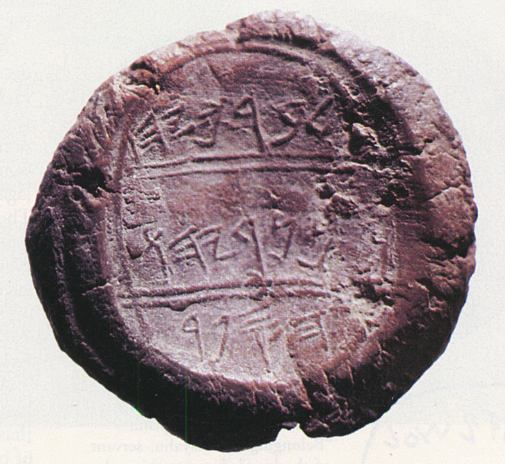
\includegraphics[scale=0.3]{Baruch_Siegel}
    \caption{Tonsiegel}
    \label{fig:Siegel}
\end{wrapfigure}

Richard Elliot Friedmann stellt die gewagte These auf, dass der Autor des Buches Jeremia dieser Autor sei. Dafür kommen laut ihn Jeremia selbst und sein Gefährte Baruch infrage. Er begründet dies textanalytisch mit einen Vergleich der Stile und Aussagen in der Deuteronomischen Historie und dem Buch Jeremia. Da Jeremia auch ein levitischer Priester in Anatoth war, dessen Vater der Finder der Buch der Thora sein könnte, nahm Friedmann dies als Grund dieser Annahme. Es ist bekannt, dass sie sehr viele seiner Lehren und Botschaften schriftlich niedergeschrieben haben. Auch wurde um 1980 von Nachman Avigad einen Siegelabdruck mit Ton gefunden, welche die Inschrift ``\textit{Eigentum von Baruch, dem Schreiber}'' trug (siehe Abb.\ \ref{fig:Siegel}). Da Jeremia und Baruch eine (vielleicht auch nur geschäftliche) Beziehung über eine längere Zeitspanne pflegten, mussten sie sich in ihren Interessen und vor allen in ihren religiösen Überzeugungen ähneln, da es sonst langfristig zu Konflikten geführt hätte, welche sich in den Schriften in Form eines stilistischen Bruchs widergespiegelt hätte. Da dieser Bruch nicht vorhanden ist, ist anzunehmen, dass zwischen Jeremia und Baruch im Inhalt ein gemeinsamer Konsens besteht. Man kann also beide als eine Einheit beurteilen. Ob Jeremia nun der ``wirkliche''  Autor ist oder nicht, spielt keine primäre Rolle.

\section{Chronistisches Geschichtswerk}
Ähnlich wie bei der Deuteronomischen Historie nimmt man an, dass die 1./2. Chronik sowie Esra und Nehemia von einen Autor geschrieben wurden und ursprünglich eine Einheit bildeten. Diese These war weitestgehend akzeptiert, wird jedoch immer mehr hinterfragt. Die Frage nach dem Verfasser ist also immer noch offen.
\\~\\
Auch wenn die Schriften textanalytisch sowie theologisch Gemeinsamkeiten aufweisen, gibt es in manchen Stellen Spuren von einer nachträglichen Bearbeitung. Eine Theorie ist, dass es einen Urautor 400 v. Chr.\ gab, der den Urtext schrieb und einen jüngeren Chronisten um 300 v. Chr., der den Urtext erweiterte, ähnlich wie Jeremia im Deuteronomischen Geschichtswerk. Diese These wird von Exegeten eher gemieden, jedoch könnte sie sowohl die Gemeinsamkeiten als auch die Unterschiede erklären.
\\
Die Frage nach dem Autor ist nicht geklärt. Jedoch kommt die aaronitische Priesterschaft infrage, da diese so schlussendlich sich ihre alleinige Macht nach dem Exil sicherte. Es ist zwar keine offizielle These und hat keinerlei Gefolgschaft, jedoch könnte Esra, gestützt auf der Annahme, dass er das Pentateuch zusammengefügt hat, das chronistische Geschichtswerk geschrieben haben. Er war ein Schriftgelehrter und genoss die Zuneigung der babylonischen Monarchie. Er besaß die Mittel und Fähigkeiten, diese Schriften abzufassen und (in einen gewissen Rahmen) um seine Interessen zu erweitern. Er könnte der Autor des Urtextes sein. Ein aaronitischer Priester könnte dann später die Schrift modifiziert haben, um Zweifel auszuräumen und/oder die Macht der Priester zu sichern oder auszubauen.
\\~\\
Zugegeben, das sind sehr, sehr weit her gegriffene Spekulationen, doch sie sind plausibel und würden sich in das bisherige Bild einfügen. Jedoch könnte es auch eine jede andere beliebige Person geschrieben haben, die literarische Fähigkeiten besaß und sich mit der damaligen Situation abfand. Wie fast im ganzen Alten Testament ist die Verfasserfrage auch hier umstritten und ein Konsens ist nicht abzusehen.

\section{Ketubim/Die Schriften}
Zu den Ketubim zählen das Buch Hiob, die Psalmen, die Sprüche, die Prediger und Hoheslied. Laut Verfassertradition wurden einige der Bücher von König Salomo geschrieben, jedoch wird heutzutage anderes angenommen. Die Verfasserfrage ist hier so schwammig, dass nur gesagt werden kann, dass die Autoren selbstständig waren. Sicherlich war der eine oder andere bereits bekannte Autor beteiligt oder die eine oder andere historische Person, jedoch kann die Verfasserfrage keineswegs geklärt werden. Man könnte dies beklagen oder die Schriften als schlichte Poesie sehen. Dies bleibt jeden selbst überlassen.

\section{Die großen Propheten}
\subsection*{Jesaja}
Die Verfasserfrage ist umstritten. Die klassische Darstellung unterteilt die Schrift in einen Protojesaja (Kapitel 1--39), einen Deuterojesaja  (Kapitel 40--55) und einen Tritojesaja (Kapitel 56--66) und ordnet allen drei Teilen einen eigenen Verfasser zu. Dies fußt auf der rationalen Annahme, dass keine Prophetie über die Lebenszeit hinweg möglich sei und dass es anscheinend schwerwiegende textanalytische Unterschiede gäbe. Jedoch ist zu kritisieren, dass für eine Schrift mit irrationale Gegebenheiten wie z.B. die Prophetie rationale Maßstäbe angewandt werden. Aus Standpunkt eines Glaubenden können Prophetien sehr wohl möglich sein und die Theologie ist eine Wissenschaft, die nicht komplett vom Glauben getrennt werden kann.
\\~\\
Die andere Theorie verfechtet diese Aufteilung und sieht die Schrift als eine Einheit an. Prophetie sei möglich und schon öfters im Alten Testament eingetreten. Auch reden Zeitzeugen und andere Schriften wie z.B. die Septuaginta immer von einen einheitlichen Jesaja. Die stilistische Unterschiede müssen auch nicht gegen eine einzigen Verfasser sprechen. Es gibt genug gemeinsame stilistische Merkmale und die stilistischen Unterschiede schließen einen einheitlichen Jesaja nicht aus. Goethes Faust I und II weisen auch stilistische Unterschiede auf und haben trotzdem zweifellos denselben Verfasser. Das gleiche kann auch auf Jesaja übertragen werden. Jesaja selber ist also der Verfasser des gleichnamigen Buches. Jesaja stammte aus einer vornehmen, judäischen Familie, wurde ca. 765--760 v. Chr.\ geboren und pflegte Kontakte zum König Usija und zu einen Priester. Er wurde von Gott berufen und ist somit göttlich inspiriert.

\subsection*{Jeremia}
Das Buch des Jeremia wurde 605/604 v. Chr.\ von den Propheten Jeremia selbst geschrieben. Jedoch diktierte er es seinen Schreiber Baruch, der es verschriftlichte. Die Übersetzungen der Septuaginta sind um ein Achtel kürzer und unterscheidet sich in der Anordnung der Kapitel als die originale hebräische Fassung, da die Übersetzer offenbar Wiederholungen raus kürzen und die Geschichten in eine chronologische Reihenfolge ordnen wollten. Die göttliche Inspiration Jeremias steht außer Frage, da Jeremia Priester war und von Gott persönlich berufen und geleitet wurde.

\subsection*{Klagelieder}
Die Klagelieder sind anonym geschrieben. Aufgrund eines ähnlichen Stils und des passenden historischen Hintergrundes ist man lange zeit davon ausgegangen, dass Jeremia der Verfasser sei. Dies ist heutzutage jedoch umstritten. Jeremia kann der Autor sein, muss es aber nicht. Die Argumente dafür und dagegen halten sich in der Waage. Da dies ein poetisches Buch ist, spielt die offene Verfasserfrage kein gravierende Rolle.

\subsection*{Ezechiel/Hesekiel}
Ezechiel war ein Priester und Prophet zur Zeit der babylonischen Verbannung. Das Buch wurde zweifelsfrei von ihm selber geschrieben. Er nennt sich selber als Autor und die Schrift hat einen durchgängig einheitlichen Stil, die einen Priester wie Ezechiel zugeordnet werden kann. Das Buch wurde 592--570 v. Chr.\ in Babylonien geschrieben. Wie Jeremia ist Ezechiel aufgrund seines Priesteramtes und seiner göttlichen Berufung göttlich inspiriert.

\subsection*{Daniel}
Bei Daniel teilen sich die Ansichten wie bei Jesaja in zwei Lager auf. Ähnlich wie bei Jesaja ist ein Grund dafür, dass Prophetie über die Lebenszeit hinaus nicht möglich sei. Mit der bereits getroffenen Annahme, dass Prophetie möglich ist, ist anzunehmen, dass der Verfasser auch wirklich der Prophet Daniel ist.Außerdem ist Daniel ein perfektes Beispiel für die Prophetie über die Lebenszeit hinweg, da Daniel bis zu der Zeit Jesus prophetiert bzw.\ einen Traum gedeutet hat. Da aber der alttestamentliche Kanon mit der Septuaginta bereits vor Jesus vollendet war, kann diese Prophetie nicht nachträglich eingefügt worden sein. Die Schriftrollen von Qumran kennen auch nur einen einheitlichen Daniel.  Es gibt Verbindungen von damaligen babylonischen Machthabern zu Daniel, deren Existenz nachgewiesen ist. Diese werden im Buch Daniel  genannt und lassen somit eine Datierung zur Zeit des Babylonischen Exils deuten. Das Buch wurde somit vermutlich um 535 v. Chr.\ in Babylonien verfasst. Daniel wurde nicht im klassischen Sinne berufen, erhielt jedoch die Gabe der Traumdeutung und war ein ergebener Diener Gottes. Man kann daher davon ausgehen, dass Daniel göttlich inspiriert war.

\section{Dodekapropheton/Kleine Propheten}
\subsection*{Hosea}
Das Buch Hosea ist eines der am schlechtesten erhaltenen Bücher. Über Hosea selber ist wenig bekannt. Die einzige Quelle über seine Person ist seine eigene Schrift. Dies lässt Zweifel zu, dass Hosea selber das Buch als eine Einheit geschrieben hat. Die Entstehung dieser Schrift ist heutzutage sehr umstritten. Es kann jedoch davon ausgegangen werden, dass weder die These, das Buch sei von Hosea selber geschrieben worden noch die These, das Buch sei eine Komposition vieler jüdischer Schriften nicht gehalten werden können. Als minimaler Grundkonsens lässt sich festhalten, dass das Buch in seiner überlieferten Gestalt eine in mehreren Phasen gewachsene planvolle Komposition darstellt. Dabei  ist es auch wahrscheinlich, dass einige Passagen auf die Reden des Hosea zurückgehen. Es ist anzunehmen, dass das Buch seine Endgestalt in Juda erhalten hat. Aufgrund der schwammigen Verfasserfrage lassen sich nur wage Rückschlüsse auf die göttliche Inspiration treffen. Es ist jedoch anzunehmen, dass Hosea und die späteren Redaktoren nach der Wahrheit Gottes gesucht hatten, d ihre Klageschriften nach Gott suchen. Es ist also möglich, dass sowohl die Autoren als auch die Redaktoren göttlich inspiriert waren.

\subsection*{Joel}
Das Buch Joel ist zweifelsfrei auf Joel selber zurückzuführen, da Petrus ihn in der Apostelgeschichte zitiert. Strittig ist die Einheit des Buches. Während die einen die Einheit befürworten, teilen die andern das Buch in zwei Teile auf, nämlich Kapitel 1 und 2 und Kapitel 3 und 4. Dies spielt jedoch eine untergeordnete Rolle, das beide Bücher zweifelsfrei auf Joel zurückzuführen sind. Auch die Datierung ist sehr umstritten und spaltet sich von der frühe vorexilischen Zeit um 800 v. Chr.\ bis zur spät-nachexilischen Zeit um 200 v. Chr.\ auf. Da es keinen König gab, bei dem der Zentralkult verehrt wurde und der Autor für die Zeit typische, aramäische Begriffe benutze ist es anzunehmen, dass Joel 400--300 v. Chr.\ geschrieben wurde. Über den Verfassungsort lässt sich keine Aussage treffen. Seine Ausdrucksweise  deutet daraufhin, dass er für sein Volk betete und laut der Überlieferung war er von Gott berufen. Folglich war Joel göttlich inspiriert, auch wenn wir wenig über seine Person wissen.

\subsection*{Amos}
Heutzutage ist die Entstehungsgeschichte zu Amos umstritten. Es wird angenommen, dass die Schrift mindestens einer Redaktion durchlaufen ist, seine Endfassung das Produkt einer nachexilischen Ära sei und drei verschiedene Profile aufweist (Am 1--2, Am 3--6, Am 7--9). Die Überlieferungen werden auf Amos zurückgeführt, jedoch sind Kapitel 1,9, Kapitel 1,11f.; Kapitel 2,4f.; Kapitel 3,7;  und Kapitel 9,8--15 nicht Amos zuzuschreiben. Umstritten ist, ob Kapitel 5,6, Kapitel 5,14f, Kapitel 8,4--7 und Kapitel 8, 11--14 auf Amos zurückzuführen sind. Die möglichen Verfasser der genannten Stellen könnten jedoch mit hoher Wahrscheinlichkeit Schüler oder Nachfolger Amos sein, die sein Werk erweitern oder neu interpretierten. Folglich wären sie genauso wie er gläubig und es ist wahrscheinlich, dass Gott sie genauso geleitet hat wie Amos selber, um eine Schrift nach seinen Vorstellungen zu gewährleisten. Die Stellen, die auf Amos zurückzuführen sind, sind aufgrund seiner Berufung göttlich Inspiriert. Bei den anderen Stellen kann keine eindeutige Aussage getroffen werden, jedoch ist eine Tendenz hin zur göttlichen Inspiration möglich. Zum Glück stammen nur wenige Verse von ihnen, sodass es nicht schwer ins Gewicht fällt.

\subsection*{Obadja}
Die Entstehung wird verschieden konstruiert. In der Regel geht man davon aus, dass Obadja in einen mehrstufigen Prozess geschrieben wurde. Dabei geht Zenger von einer dreistufigen Entstehungsprozess aus, der in der ersten Hälfte des 6. Jh v. Chr.\ anfing und am 3./4. Jh v. Chr.\ beendet wurde.	Wöhrle dagegen proklamiert bist au 17a auf einen einheitlichen Text, der in der frühhellenistischen Zeit (3. Jh v. Chr.) geschrieben wurde. Ersteres ist plausibler. Demnach wäre die erste Stufe auf Obadja zurückzuführen. Über Obadja weiß man sehr wenig. Genauso wenig weiß man, wer die anderen zwei Stufen geschrieben hat. Man kann die Autoren auf Israel eingrenzen, da Edom in dieser Schrift negativ dargestellt wird und sich ein israelitischer Autor aufgrund des Völkerkonfliktes zwischen Edom und Israel perfekt in das Bild einfügen würde. Da über die Autoren wenig bekannt ist, lassen sich keine eindeutige Aussagen über ihre göttliche Inspiration treffen. Man könnte darauf spekulieren, dass sie Juden, aufgrund ihrer schreiberischen Fähigkeiten höher gebildet und/oder deswegen Schriftgelehrte oder Priester waren, jedoch gibt es dafür keinerlei Beweise.

\subsection*{Jona}
Jona selber bezeichnet sich selbst nie als Prophet noch versteht sich die Schrift als Prophetenschrift. Die Schrift ist daher eine Prophetenerzählung in Prosaform. Eine textanalytische Analyse ergibt, dass die Schrift in der nachexilistischen Zeit anzusetzen ist. Spezifischer wird die Datierung zwischen der Perserzeit im 5. Jahrhundert v.Chr.\ bis in die hellenistische Zeit im 3. Jahrhundert v.Chr.\ angesetzt. Da aber in Jesus Sirach, eine Schrift in den Apokryphen, der Dodekapropheton erwähnt wird, in dem Jona mitvertreten ist, kann eine Datierung früher als 200 v.Chr.\ nicht möglich sein. Aufgrund der im Verschlingungsepisode und im Ninivebild aufgenommenen außerbiblischen Traditionen ist eine Datierung in die hellenistische Zeit wahrscheinlicher. Bei beiden Datierungen steht jedoch Jona als Verfasser selbst außer Frage. Längere Zeit zweifelte man die Einheitlichkeit der Schrift an, jedoch wird heutzutage die Einheit der Schrift -bis auf den eingeschobenen Psalm- nicht mehr angezweifelt.
\\~\\
Die teils sehr phantastischen Erzählungen beweisen, dass die Schrift nicht als historische Schilderung verstanden werden will. Daher stellt sich nur die Frage, ob die Botschaft selber göttlich inspiriert sei. Hier lassen sich nur wage Aussagen treffen. Da das Buch sehr wahrscheinlich zur Belehrung dient, ist es durchaus möglich, dass ein Schriftgelehrter oder ein Priester diese Schrift geschrieben hat, da diese das Wissen, die Fertigkeiten und die Autorität dazu besaßen. Da diese eine außerordentliche Verbindung zu Gott besaßen und nach seinen Willen agieren wollten, ist eine göttliche Inspiration möglich. Jedoch wissen wir anhand der Evangelien und den Geschichten rund um Jesus, dass diese -freiwillig oder unfreiwillig- auch mal entgegen Gottes Vorstellungen agierten. Die Botschaft der universalen Gnade Gottes, die auch von Jesus gelehrt wurde, beseitigt in diesen Fall die Zweifel.

\subsection*{Micha}
Das Buch Micha unterlief einen teils komplexen Entstehungsprozess, der wahrscheinlich 500 Jahre gedauert hat. Das Buch unterlief vermutlich einen fünfstufigen Entstehungsprozess, in dem die Worte des Propheten Micha aktuell blieben und lediglich neu verstanden bzw.\ neu interpretiert wurden. Der Entstehungsprozess begann im 8. Jahrhundert v.Chr.\ mit den Feldzug Sargons II.\@ gegen Philistäa und endete vermutlich in der ptolemäische Zeit im 3. Jahrhundert v.Chr.
\\~\\
Der älteste Teil des Michabuchs findet sich in Mi 1--3, wobei nach der neuesten Forschung davon auszugehen ist, dass selbst hier keine bloße Zusammenstellung von authentischen Michaworten vorliegt, sondern die Anliegen des historischen Micha durch einen Schüler- oder Sympathisantenkreis literarisch verarbeitet wurden. Diese so genannte ``Micha-Denkschrift'' aus dem 7. Jahrhundert v.Chr.\ wurde nach der Katastrophe von 586 v.Chr.\ durch 4,8--5,3 ergänzt und frühnachexilisch zu der Komposition Mi 1--5 erweitert. Mitte des 5. Jahrhundert v.Chr.\ kam die Komposition 6,1--7,7 hinzu. Im Rahmen der Endredaktion am Ende der persischen Zeit bzw.\ zu Beginn des hellenistischen Zeitalters (4./3. Jahrhundert v.Chr.) wird der Schluss des Michabuchs Mi 7,8--20 erstellt. Entsprechend der Abfolge ``Unheil-Heil'' zeigt sich für beide Teile (1, 2--5, 14 und 6, 1--7, 20), dass die Heilsperspektive jeweils eine Aktualisierung der älteren Unheilsperspektive darstellt.
\\~\\
Da der Grundbestand der Schrift auf Micha selber, einen Propheten zurückzuführen sind und die Redakteure das Ziel hatten, Gottes Worte, die durch Micha kundgetan wurden, für ihre Zeit zu deuten und zu interpretieren, ist anzunehmen, dass sowohl der Grundtext nach Micha als auch die späteren Ergänzungen göttlich inspiriert sind bzw.\ sich vom heiligen Geist haben leiten lassen.

\subsection*{Nahum}
Das Buch Nahum weist einen mehrstufigen Entstehungsprozess auf. Die Entstehung begann zw. 664--612 v.Chr.\ und endete im 4. Jahrhundert v.Chr.. Der erste Teil der Schrift wurde zur Zeit des Untergangs Thebens bis zum Untergang Ninives geschrieben. Wann die weiteren Fortschreibungen Nahums historisch zu verorten sind, ist schwer zu bestimmen. Vereinfacht lässt sich sagen, dass Nahum in zwei Blöcken geschrieben wurde. In einen richtet es sich an Ninive und dessen Zerstörung, also an den zuvor datierten Block, und im anderen an Juda selber. Letzterer Block kam zu der Zeit des Babylonischen Exils hinzu.\ in der nachexilischen Zeit wurden diese Blöcke redaktionell verwoben und um den Psalm erweitert.
\\
Da wenig über den Entstehungsprozess bekannt ist, lässt sich nur die Aussage treffen, dass die Worte, die direkt auf Nahum zurückzuführen sind, göttlich inspiriert sind, da er von Gott berufen wurde und er seine Worte verkündete. Da aber die Redaktion vermutlich nur zwei Quellen verwoben hat, ist anzunehmen, dass es sich bei den zwei Quellen um zwei verschieden Überlieferung (-sgeschichten) handelt, die beide Nahum als sprachliche Quelle als Ursprung haben und sich über verschiedene Wege verschriftlichten, bis sie zu einer Einheit zusammengefügt wurden. Daher wird die ganze Schrift göttlich inspiriert sein, da beide Blöcke auf Nahum zurückzuführen sind.

\subsection*{Habakuk}
Die Entstehung wird zwischen 625 v.Chr.\ und 605 v.Chr.\ datiert. Er hat sein Buch vermutlich in Juda verfasst, da Habakuk nicht unter der Zerstörung des Nordreiches litt. Nach dem Fund eines Kommentars zu den Buch habakuk in den Qumranhölen zweifelte man die Einheit des Buches an, da in diesen Kommentar nicht Zefanja 3 erwähnt wurde. Jedoch sind diese Vorwürfe abzuschmettern, da sich in Zefanja 1--3 textanalytisch grammatikalische, sprachliche und thematische Zusammenhänge festgestellt werden konnten. Jedoch unterlief die Schrift mehrerer Redaktionen, in denen auch geringfügige Ergänzungen gemacht wurden. So wurde einzelne Ergänzungen gemacht, um das Buch in das Dodekapropheton einzufügen und um ein ganzes Anti-Babylonisches Werk zu kreieren. Eine solche Ergänzung wären z.B. die Weherufe und Klagen. Auch wurden einzelne stilistische Eingriffe unternommen, um so die Schrift in einen Gottesdienst gebrauchen zu können. Letztendlich ist der Grundbestandteil aber auf Habakuk selbst zurückzuführen und wurde nur um liturgische und kleinere thematischen Aspekte erweitert oder neu interpretiert. Daher ist auch hier davon auszugehen, dass ähnlich wie bei Micha Habakuk selbst als Prophet als auch die Redaktoren göttlich inspiriert waren.

\subsection*{Zefanja}
In der neueren Forschung ist die Annahme weithin akzeptiert, dass das Zefanjabuch aus einer Reihe literarischer Einheiten zusammengesetzt ist und einen mehrschichtigen Redaktionsprozess verrät.Die ältesten Teile des Buches werden in die Zeit des Reformerkönigs Joschija von Juda in der zweiten Hälfte des 7. Jahrhunderts v.Chr.\ datiert. Seine jüngste Teile stammen aus dem 4./3. Jahrhundert v.Chr. Es ist anzunehmen, dass einige der früheren Textpassagen auf Zefanja selbst zurückgehen. Spätere Ergänzungen sind einerseits auch auf Zefanjas Worte zurückzuführen und andererseits redaktionellen Erweiterungen im babylonischen Exil, um das eingetretenen Gottesgericht über Juda zu dokumentieren und zu begründen. In der nachexilistischen Zeit wurden Heilsversprechungen eingefügt und das Gottesgericht universalisiert.
\\
Da durch die späteren Redaktionen das ursprüngliche Wort Zefanjas unberührt blieb und nur um weitere Aspekte erweitert wurde, ist anzunehmen, dass die Schrift göttlich inspiriert ist. Ähnlich wie bei dem Buch Micha ist anzunehmen, dass die Redaktoren göttlich inspiriert sind, weil sie bei den offenen Fragen sich von Gott haben leiten lassen.

\subsection*{Haggai}
Viele Forscher nehmen an, dass Haggai kurz nach seinen Auftreten entstanden ist. Es ist jedoch anzunehmen, das literarisch ein paar wenige Eingriffe eines Redakteurs unternommen wurden. Der Inhalt an von sich ist aber auf Haggai bzw.\ seine Reden selbst zurückzuführen. Daher ist die Datierung um um 620 v.Chr.\ anzusiedeln, da dort die Reden Haggauis präzise in der Schrift selber datiert wurden. Da Haggai ein Prophet war und somit von Gott berufen und eingesetzt, ist das Buch göttlich inspiriert, da die eingriffe rein stilistischer Natur sind.

\subsection*{Sacharja}
Das Buch Sacharja wird in in eine Proto- und Deuterojesaja eingeteilt. Ersteres umfasst Sacharja 1--9 und ist zweifelsfrei auf ihn selbst zurückzuführen. Letzteres war wahrscheinlich eine Ergänzung eines späteren Propheten, dessen Wirken zusammen mit Sacharjas zu einer Sinneseinheit zusammengefügt wurden. Der Protosacharja ist 520--518 v.Chr.\ zu datieren und der Deuterosacharja wird in die hellenistische Zeit im 3./2. Jahrhundert v.Chr.\ datiert. Da beide Schichten thematische Gemeinsamkeiten aufweisen, ist anzunehmen, dass der Verfasser des Deuterosacharja die Aussagen des Sachaarja erweiter bzw.\ vollendet hat. Daher ist anzunehmen, dass beide als Propheten oder als Prophet und als Verfasser, dessen Aussagen die eines Propheten entsprechen göttlich inspiriert sind.

\subsection*{Maleachi}
Zunächst nahm man an, dass Maleachi nicht als Name, sondern als ein Buchtitel verstanden werden muss und eine Gruppe diese Schrift verfasst habe. Heutzutage zieht man jedoch Maleachi als ein Prophet in Betracht, belegt wurde diese These jedoch nicht und wird aufgrund fehlender Belege nie belegt werden können. Die Entstehung ist eine offene und schwierige Frage. Es gibt jedoch eine Grundschicht, die auf Maleachi selbst zurückgeführt werden kann. Diese wurde dann unsystematisch um einzelne Worte ergänzt. Dadurch lassen sich spätere Redaktoren praktisch nicht ermitteln. Die Frage nach der göttlichen Inspiration ist also schwammig beantwortbar. Die Grundschicht wird aufgrund dessen, dass Maleachi als Prophet berufen war, göttlich inspiriert sein, jedoch lässt sich keine Aussage über die Redaktoren treffen. Diese scheinen aber die Schrift um nur einige Gesichtspunkte erweitert zu haben, jedoch in keiner Weise, dass ganze neue Aspekte geschaffen wurden.


\section{Schlussbetrachtung}
Die Entstehungsprozesse der einzelnen Schriften sind teilweise sehr Komplex und weisen gerade im Dodekapropheton einen vielschichtigen und komplexen Entstehungsprozess auf, der hier nur auf das simpelste runter gebrochen wurde. Einige Schriften wie z.B. das Pentateuch, aber auch des Deuteronomischen Geschichtswerkes sind extrem Kontrovers und die eine Wahrheit gibt es bei dieser Thematik nicht. Glücklicherweise konnten meistens die Grundbestandteile der Schriften auf Propheten oder andere von Gott berufene Persönlichkeiten zurückgeführt werden, sodass der Kern göttlich inspiriert ist. Die Grundtheologien der einzelnen Schriften blieben unverändert.
\\~\\
Doch in den meisten Fällen steckt noch eine langwierige Redaktionsgeschichte dahinter, die von den aktuellen historischen Ereignissen geprägt wurden. Gerade wenn es um Ergänzungen von Schriftgelehrten oder Priestern geht, die v.a. Gesetze, Bräuche oder Machtverhältnisse beinhalten, muss die Schrift kritisch betrachtet werden. Nicht selten versuchten Eliten, durch gezielte Geschichtsschreibung die Missstände zu verdecken, auch wenn größere Lügen hier nicht entdeckt wurden oder an anderen Stellen der Bibel richtig gestellt werden.
Ein großer Knackpunkt vor allen bei den großen Propheten sind die Einheit einzelner Bücher. An Stellen wie z.B. dem Pentateuch ist es angebracht, jedoch werden durch fragwürdige Annahmen z.B. Bücher wie Jesaja aufgeteilt. Schlussendlich muss sich aber jeder selber entscheiden, ob er an einer Einheit oder einer Aufteilung der Schriften festhält.
\\~\\
Erstaunlich ist, wie bei Entstehungsgeschichten, die sich teilweise über ein halbes Jahrtausend erstreckten, der Kernbestand unverändert blieb und immer auf eine von Gott eingesetzte, berufene oder geleitete Person zurückführen lässt. Die Ergebnisse stellen auf den ersten Blick die Glaubwürdigkeit des Alten Testaments in Frage, jedoch gibt es im Vergleich zu anderen Werken kein vergleichbares Werk von Geschichtsschreibung. Das Alte Testament ist für die damaligen Verhältnisse als Geschichtsschreibung präzise und einzigartig! Natürlich Bedarf es bei der Exegese eine grundkritische Einstellungen, um Fehler durch Menschenhand ausfindig zu machen. Letztendlich bleibt die Bibel Gotteswort in Menschenwort und Menschenwort ist fehlbar.
\chapter{Das Neue Testament}
Ein römischer Kleriker behauptete, dass die Existenz Jesu historisch bewiesen sei. Darauf folgte Kritik und sogar eine Anzeige, welche sich jedoch verlaufen hat. Auch wenn die katholische Hierarchie fragwürdig ist, ist diese  Aussage jenes Glaubensbruders sehr zutreffend. Die Existenz Jesu ist mehrfach überliefert und bewiesen, auch von dritten, unabhängigen Quellen. Es folgen ein paar Exzerpte:
\medskip
\begin{center}
    \begin{minipage}{0.9\linewidth}
        \small
        ``Christus war unter des Tiberius Führung vom Procurator Pontius Pilatus hingerichtet worden''
        \\ \footnotesize{\textit{(Cornelius Tacitus, Annalen, Phaidon Verlag, Wien 1935, S 740; XV.\@ 44)}}\small
        \\~\\
        „Um diese Zeit lebte Jesus, ein weiser Mann, wenn man ihn überhaupt einen Menschen nennen darf. Er vollbrachte nämlich ganz unglaubliche Taten und war der Lehrer aller Menschen, die mit Lust seltsame Dinge aufnahmen. So zog er viele Juden und auch viele Heiden an sich. Dieser war der sogenannte Christus. Und obgleich ihn Pilatus auf Betreiben der Vornehmsten unseres Volkes zum Kreuzestod verurteilte, wurden doch seine früheren Anhänger ihm nicht untreu. Denn er erschien ihnen, wie sie behaupteten, am dritten Tage wieder lebend, wie gottgesandte Propheten dies und tausend andere wunderbare Dinge von ihm vorhergesagt hatten. Und bis auf den heutigen Tag besteht das Volk der Christen, die sich nach ihm nennen, fort.“
        \\ \footnotesize \textit{(Flavius Josephus, Antiquitates Judaicae, Verse 63–64)} \small
        \\~\\
        Im Britischen Museum befindet sich das Manuskript eines Briefes, der etwa 73 n. Chr.\ von einem Syrer namens Mara Bar-Serapion verfasst worden ist. Er erwähnt die Hinrichtung von Sokrates, Pythagoras und Christus und zeigt, dass die Verfolgung von weisen Männern nur Unglück bringt.
        \\ \footnotesize \textit{(F. F. Bruce, Die Glaubwürdigkeit der Schriften des Neuen Testaments, Verlag der Liebenzeller Mission, 1976, S. 122)} \small
        \\~\\
        Lucian, ein Satiriker des 2. Jh.\ n. Chr.\ bezeichnete Jesus als ``den in Palästina gekreuzigten Menschen''
        \\ \footnotesize \textit{(Lucian, Über das Lebensende des Peregrinus, in Lucian Bd. 2, S. 9, Griechische und römische Klassiker, Langenscheidt Verlag, Berlin 1855--1920, Bd. 36)} \small
        \\~\\
        ``Da die Juden unter ihrem Anführer Chrestos (d.h. Christus) beständig Unruhe anstifteten, vertrieb er (d.h. Claudius) sie aus Rom''
        \\ \footnotesize \textit{(Gaius Suetonius Tranquillus, Leben der Caesaren, Claudius, Artemis-Verlag, Zürich 1955, S. 296; § 25)} \small
    \end{minipage}
\end{center}

\begin{center}
    \begin{minipage}{0.9\linewidth}
        \small
        Um 150 n. Chr.\ schickte Justin der Märtyrer eine Verteidigungsschrift des Christentums an Kaiser Antonius Pius und verwies ihn an den Bericht des Pilatus, der in den kaiserlichen  Archiven aufbewahrt wurde: ``Dass dies so geschehen ist, könnt ihr aus den unter Pontius Pilatus angefertigten Akten ersehen''
        \\ \footnotesize \textit{(Justin der Märtyrer, Apologien, Kösel Verlag, München 1913, S 48 f.u. 61; I.35)} \normalsize
    \end{minipage}
\end{center}
\medskip
Egal, ob diese Überlieferungen zweifelsfrei sind oder nicht, allein der Fakt, dass so viele Quellen -viele davon aus dritter Hand- von Jesus berichten, bestätigen dessen Existenz. Manche gehen soweit, dass sie sagen, dass man die Evangelien aus dritten Quellen fast komplett rekonstruieren könne. Die Gefolgschaft Jesu war zahlenmäßig groß und so auch die Überlieferungen. Schlussendlich gibt es mehr Quellen, die Jesus Existenz und somit sein wirken bestätigen als bei Gaius Julius Cäsar, dessen Existenz und Geschichten nicht angezweifelt werden. Heutzutage \emph{weiß} man, dass Jesus existiert hat.


\section{Die synoptischen Evangelien}
\begin{figure}[h]
    \begin{center}
        
\includegraphics[width=\linewidth]{Zwei-Quellen-Theorie}\label{Quellentheorie}
        \caption{Schematisches Schaubild der Zwei-Quellen-Theorie}
    \end{center}
\end{figure}
Die am meisten anerkannte und plausibelste Theorie für die Überlieferung der synoptischen Evangelien ist die sogenannte Zwei-Quellen-Theorie. In dieser wird angenommen, dass eine frühere Fassung des Markus-Evangeliums (Urmarkus) die älteste Überlieferung darstellt und sowohl Lukas als auch Matthäus als Basis gedient haben. Dies erklärt auch die meisten Übereinstimmungen zwischen Markus, Lukas und Matthäus.\\

Jedoch gibt es auch (teilweise wortwörtliche) Übereinstimmungen  zwischen Lukas und Matthäus, welche jedoch nicht im Markus-Evangelium vorkommen. Dies wird durch die hypothetische Größe der Logienquelle erklärt. Diese vermutlich schriftliche Quelle soll den beiden Evangelisten als zweite Quelle gedient haben, welche Markus nicht zugänglich war und beschränkt sich größtenteils auf die Sprüche bzw. Reden Jesu. Jedoch wurde bis heute diese Quelle nicht gefunden und muss über die Zeit durch Verwitterung, Verfall und mutwillige Zerstörung durch z.B. Krieg vernichtet worden sein. Solange diese Quelle nicht geborgen wird, wird diese Theorie ein Erklärungsversuch ohne Beweis bleiben.\\

Zuletzt besitzen sowohl das Lukas- als auch das Matthäusevangelium beide Passagen, die in den anderen Evangelien nicht vorkommen. Dies wird mit weiteren Quellen, dem Sondergut erklärt. Dies sind mündliche oder schriftliche Quellen, auf die nur die jeweiligen Verfasser Zugriff hatten. Auch diese wurden noch nicht gefunden und sind hypothetische Größen.
\\~\\
Die wohl größte Schwäche sind die hypothetischen Quellen, welche nicht erhalten sind. Jedoch ist die Annahme einer gemeinsamen Logienquelle und der Sondergüter plausibel, da alle Verfasser sich verschiedener Quellen bedienen mussten. Deutlich wird dies am Anfang des Lukas-Evangeliums, in dem Lukas davon berichtet, wie er die verschiedenen Quellen zusammengetragen und verschriftlicht hat. Und da damals die Anzahl der Überlieferungen limitiert waren, ist die Wahrscheinlichkeit einer gemeinsamen Logienquelle groß. Wie sich heute jeder Schüler bei einer Recherche bei einer gemeinsamen Quelle namens Wikipedia bedient und dann noch zusätzlich weiterer Quellen, so bedienten sich damals Lukas und Matthäus einer gemeinsamen Quelle X und ihrer eigenen zusätzlichen Sonderquellen.\\

Ein weiterer Kritikpunkt ist, dass im Markus-Evangelium Passagen aufzufinden sind, die von Lukas und Matthäus nicht übernommen wurden. Ein Grund kann sein, dass diese Passagen nach dem Verfassen der anderen Evangelien hinzugefügt worden sind und heutzutage eine überarbeitet Fassung (Deuteromarkus) des Urtextes (Urmarkus) vorliegt. Auch erklärbar sind diese Passagen als redaktionelle Gründe von Lukas und Matthäus, weil sie z.B. als anstößig empfunden wurden. Jedoch erklärt dies nicht alle Passagen und es ist schwierig, eine befriedigende und anerkannte Antworten für dieses Problem zu finden.\\

Der letzte nennenswerte Kritikpunkt sind die Minor agreements. Diese sind Passagen, die bei Lukas und Matthäus übereinstimmen, sich jedoch zu Markus unterscheiden. Dabei kann es sich um stilistische Änderungen oder Auslassungen handeln. Diese sind mit redaktionellen Gründen und stilistische Verbesserungen zu erklären. Ein weiterer Erklärungsversuch ist, dass  die Verfasser eine Urfassung (Urmarkus) des Markus-Evangeliums zur Verfügung hatten und die heutige Überlieferung eine überarbeitete Fassung (Deuteromarkus) der Schrift ist.\\

Auch wenn die 2-Quellen-Theorie nur ein ein Erklärungsversuch mit seinen genannten Schwachstellen ist, ist diese Theorie die plausibelste und erklärt am Besten die Überlieferung der drei synoptischen Evangelien. Zudem wurden zur damaligen Zeit Nachrichten, wie es heute in manchen ländlichen Gebieten auch noch üblich ist, per Mundpropaganda weitergegeben. Der Verdacht der Verfälschung ist sicherlich angebracht, jedoch konnten sich die Menschen damals die Worte fast wortwörtlich merken, da die traditionelle Mundpropaganda das Gedächtnis dazu trainiert bzw.\ getrimmt hatte.\\

Da das Lukasevangelium und das Matthäusevangelium auf der (vermutlichen) Logienquelle, den Sondergütern und dem Markus-Evangelium basieren und letzteres als einzige Quelle überliefert ist, ist das Markus-Evangelium am Besten für eine Untersuchung geeignet. Die Ergebnisse der Untersuchungen lassen sich größtenteils auf die anderen zwei Evangelien übertragen. Unbefriedigend ist der Sachverhalt, dass die zweite Quelle nicht für eine Untersuchung zur Verfügung steht. Deshalb wird ein zweite Untersuchung des Matthäus- und des Lukasevangeliums vonnöten sein.

\subsection*{Markus-Evangelium}
Laut alt-kirchlicher Überlieferung wurde das Markus-Evangelium von Johannes Markus geschrieben. Er soll der Dolmetscher von Petrus gewesen sein. Nach dieser Auffassung würde das Evangelium direkt nach Jesus Tod geschrieben worden sein und den direkten Überlieferung der Apostel zu Grunde liegen. Auch wenn es einfacher wäre, an diese Version zu glauben, gibt es Widersprüche, die dies widerlegen könnten.
\\~\\
Anzuzweifeln ist die direkte Verbindung zu Petrus. Wäre der Autor ein Dolmetscher von Petrus gewesen, hätte er von ihm wahrscheinlich mehr berichtet, da er mit ihm mehr im Kontakt als mit den übrigen Jüngern stand und es nahe steht, dass das meiste Material des Autors von Petrus hätte stammen müssen. Jedoch wird Petrus in Markus-Evangelium nicht hervorgehoben und seine Rolle wird traditionell dargestellt. Dies steht im Widerspruch zur direkten Verbindung zu Petrus. Es ist also anzuzweifeln, dass der Autor mit Petrus oder den Aposteln im engeren Kontakt stand. Die Identität des Autors ist unbekannt. Jedoch kann auf textanalytischer Basis Informationen über den Autor gesammelt werden, um den Kreis der möglichen Autoren einzuengen und Aussagen über den Autor treffen zu können.
\\~\\
Der Autor war mit großer Wahrscheinlichkeit ein Heidenchrist, d.h.\ er gehörte vor seiner Bekehrung zum (frühen) Christentum nicht dem Judentum an. Er glaubte demnach vor seiner Bekehrung nicht an den Gott Jahwe und auch nicht daran, dass eben dieser eine Gott einen Sohn auf die Erde geschickt hat, um sein Volk bzw.\ die Menschheit zu retten. Auch teilte er nicht die Geschichte Israels mit Gott. Für ihn musste vor der Bekehrung das Judentum suspekt gewesen sein, sodass er seine alte Religion beibehielt. Ihm war das Judentum fremd. Nachdem er von den Geschichten von Jesus Christus, den Messias, gehört hatte, hätte er seine alte Religion beibehalten und die Berichte anzweifeln können. Der Autor hatte mehr Gründe, die Berichte negativer aufzugreifen und darzustellen als die realen Ereignisse. Aber die Schilderungen haben anscheinend das Gegenteil bewirkt. Er hat sich vermutlich dadurch seiner eigenen Religion fremd gefühlt und dem Rücken gekehrt, einer Religion, an die er sein gesamtes Leben geglaubt hatte. Er konnte sich mehr mit Jesus Christus bzw.\ mit dem Christentum identifizieren. Seine Motivation für die Verschriftlichung war die Begeisterung für seinen neu gewonnen Glauben, der höchstwahrscheinlich sein Leben besser erfüllt hatte als seine alte Religion. Er vollzog einen Wandel von ein Kritiker zum Nachfolger Jesu. Von einer mutwilligen, ungerechtfertigten und unreflektierten Beschönigung der Bibel durch den Autor kann also kaum gesprochen werden.
\\~\\
Funde aus den Qumranhölen belegen, dass das Markus-Evangelium vor dem jüdischen Krieg (um 68 n. Chr.) entstanden sei. Die Verschriftlichung muss also davor stattgefunden haben. Im (fiktiven) Worst-Case-Szenario muss die Verschriftlichung mit der Annahme, dass der Arbeitsprozess ein Jahr dauert, 67 n. Chr.\ stattgefunden haben. Demnach würden seit dem Tod Jesu ca. 30 Jahre vergangen sein, also ca.\ eine Generation. In dieser Zeitspanne predigten die Apostel selber das Evangelium. Die Wahrscheinlichkeit liegt nahe, dass der Autor einer der Apostel begegnet ist oder zumindest zu seiner Zeit noch gelebt haben (Petrus starb vermutlich 64--67 n.Chr.). Es ist jedoch anzunehmen, dass das Markusevangelium davor geschrieben wurde.
\\
Es besteht also die Möglichkeit, dass der Autor das Evangelium direkt von den Apostel unverfälscht gehört und verschriftlicht hat. Angesichts der Bewegung der Urgemeinden und der Missionarsmissonen der 12 Apostel wäre dies nicht abwegig. Wäre dies trotzdem nicht der Fall, dann müssten die Berichte durch dritte mündlich überliefert worden sein. Folglich liegt der Verdacht der Verfälschung nahe. Da zu der Zeit die meiste Geschichten mündlich überliefert wurden, war das Gehirn dementsprechend geprägt und daran gewöhnt. Die Menschen konnten sich die Überlieferungen teilweise wortwörtlich merken und unverfälscht weitervermitteln, wie es heute in sehr ländlichen Gegenden der Erde teilweise immer noch üblich ist. Der einzige Grund zur Verfälschung wäre die Instrumentalisierung der Berichte. Jedoch war das frühe Christentum faktisch machtlos und wurde sogar verfolgt. In den meisten Regionen gab es andere Religionen, die dominanter waren. Dort wäre eine eigennützige Instrumentalisierung ertragreicher gewesen. Eine schwache Religion zu Instrumentalisieren ergibt wenig Sinn.

\subsection*{Matthäusevangelium}
Laut Verfassertradition wurde das Matthäusevangelium von den Jünger Matthäus verfasst. Ähnlich wie bei Markus ist diese Annahme vermutlich falsch und der Verfasser unbekannt. Der Autor war vermutlich ein christlicher Schriftgelehrter. Die Indizien dafür sind der Umgang mit den Alten Testament als auch der literarisch kunstvolle Aufbau des Evangeliums. Die Bibel wurde vermutlich in Syrien, genauer gesagt Antiochia geschrieben. Da in der Schrift die Zerstörung des Tempels und der judäische Krieg vorausgesetzt ist, wird die Verfassung auf 80--90 n.Chr.\ datiert.
\\~\\
In der Forschung ist die Frage umstritten, ob das Evangelium in einem juden- oder heidenchristlichen Milieu entstanden ist. Jedoch wurde die Schrift anscheinend für eine judenchristliche Gemeinde geschrieben. Auch er ist der Ansicht, dass das Heil für alle Völker gilt und kritisiert das damalige Judentum. Grund für die Kritik gab es genug. Er hat sich seiner alten Religion abgewandt und einer ``reformierten'' Fassung des Judentums (das spätere Christentum) zugewandt. Für ihn war die Lehren Jesu die Wahrheit und vor allen die Lehren der Pharisäer veraltet oder falsch. Ähnlich wie beim Markusevangelium ist es wahrscheinlich, dass der Verfasser einer der Apostel gehört hat und somit die Überlieferungen kaum verfälscht wurden. Nach der Zwei-Quellen-Theorie beruft sich Matthäus auf Markus und seinen Sondergut. Dass sich sein Sondergut direkt oder indirekt auf die Apostel beruft, ist wahrscheinlich, da die Apostel höchstens seit 30 Jahren tot sein konnten, was in einer althistorischen Schrift eine minimale Zeitspanne ist.  Auch ist das Christentum zu der Zeit faktisch machtlos, was das Argument der Instrumentalisierung der Religion entkräftet. Er hatte keinen Grund, die Schrift zu verfälschen. Er setzte lediglich nur andere Schwerpunkte in seinen Evangelium. Es ist anzunehmen, dass die Überlieferungen den Originalgeschichten entsprechen. Ausnahmen sind stilistische Ausarbeitungen wie die Symbolzahlen, welche eine Interpretation aber nur geringfügig beeinflussen können.

\subsection*{Lukasevangelium und Apostelgeschichte}
Laut Verfassertradition war Lukas ein Arzt und Begleiter des Paulus. Ob Lukas ein Schüler oder nur ein Begleiter Paulus war, ist umstritten. Jedoch verweigert Lukas Paulus den Titel des Apostel. Deswegen ist es wahrscheinlicher, dass Lukas ein Begleiter oder Freund des Paulus war. Es ist schwierig, ihn einer Gruppe zuzuordnen. Ein ärztliches Interesse lässt sich aus der Schrift nicht begründen, dennoch war er wahrscheinlich hoch gebildet. Er war also kein Arzt. Er war kein Judenchrist, da er keine semitischen Begriffe verwendet und durch griechische ersetzt. Wahrscheinlich war er ein ``Gottesfürchtiger'', welcher mit dem Judentum sympathisierte, aber sich nicht zu diesen bekehren lies. Aber mit großer Sicherheit war er wie Markus ein Heidenchrist. Die Verfassung ist um 70--90 n.Chr.\ zu datieren.
\\~\\
Wie bei Matthäus und Markus ist eine Instrumentalisierung aus den gleichen Gründen unwahrscheinlich. Er wurde vermutlich vor Matthäus und nach Markus geschrieben. Dass sein Sondergut sich auf die Apostel in erster oder zweiter Ebene beruft, ist wie bei Markus und Matthäus sehr wahrscheinlich. Auch er hatte keinen Grund, die Überlieferungen zu verfälschen.

\section{Johannesevangelium}
Das Johannesevangelium unterscheidet sich grundlegend von den synoptischen Evangelien und muss in seinen Entstehungsvorgang als eigenes Werk betrachtet werden. Dass Johannes ein Augenzeuge war, ist eher unwahrscheinlich. Dafür weist die Schrift zu reflektierende Merkmale auf. Dies spricht eher von einer zeitlichen Distanz seit dem Wirken Jesu. Die Schrift wurde vermutlich 90--100 n. Chr.\ in Syrien oder Ephesus verfasst. Der Autor stammt vermutlich aus einen judenchristlichen Milieu, da dreimal der Ausschluss aus der Synagogengemeinde als Folge des Bekenntnisses zu Jesus als dem Christus erwähnt wird. Textanalytisch kann man sagen.\ dass Johannes nicht von einer Person geschrieben wurde, sondern von einen Urautor, einer sogenannten ``johanneischen Schule'' (Kapitel 15, 16 und 17) und dem Herausgeber bzw.\ den Redakteur (Kapitel 21).
\\~\\
Der Urautor lässt sich schwer identifizieren. Vermutlich war er ein Judenchrist. Da er von den Ausschluss aus der Synagogengemeinde, sprich der Judengemeinde schreibt, liegt es nahe, dass er dies selbst erlebt haben könnte. Folglich stand er vor einer Wahl: Seine alte Religion, an die er sein bisheriges Leben geglaubt hatte, beibehalten oder sich dem neuen Christentum zuwenden. Er stand wie alle Judenchristen im Konflikt und wägte ab. Er wandte sich einer neuen Religion zu. Er befand diese für wahr. Folglich hatte er keinen Grund, sich seine neue Religion schönzureden oder zu verfälschen. Er hatte sich selbst entschieden. Es liegt nahe, dass seine Gedanken und Entscheidungsgründe für die Bekehrung in die Schrift mit eingeflossen ist. Dies würde auf den Schwerpunkt auf Jesus als Offenbarung erklären. Da das Evangelium die Struktur der synoptischen Evangelien besitzt, wird angenommen, dass der Autor diese kannte. Seine Schrift kann daher entweder als Kritik der alten Überlieferung zu sehen sein oder als Vertiefung. Auf jeden Fall soll seine Schrift eine Alternativversion der synoptischen Evangelien sein.
\\
Die johanneische Schule lebte in einen potentiell aggressiven Umfeld. Die Schule grenzt sich vom Judentum in seinen Bräuchen ab, leugnet dieses aber nicht komplett. Durch die spätere Abfassung ist es möglich, dass sowohl Johannes als auch seine Gemeinde eine zusätzliche Anzahl von Quellen, die in der Zeit um und nach der Verfassung der synoptischen Evangelien entstanden und/oder gefestigt hatten, zur Verfügung hatte. Eine zusätzliche hypothetische Quelle (-nsammlung) X ist also plausibel, jedoch gibt es keine überlieferten Manuskripte davon.
\\~\\
Die Frage der historischen Korrektheit und der Glaubwürdigkeit der Evangelien (inklusive der Apostelgeschichte) ist also geklärt. Anzumerken ist, dass es vollständige Manuskripte aller dieser Schriften gibt und die Zeitspanne zwischen dem Wirken Jesu und der Verschriftlichung verhältnisweise sehr klein ist. Die Evangelien und auch die Bibel wird oft zurecht als die historisch gesehen beste Geschichtsschreibung gesehen, trotz der Missstände im Mittelalter und der vielen Übersetzungen.

\section{Jesus Christus ist der Messias}
An Jesus Existenz und der Glaubwürdigkeit der Evangelien gibt es -wenn man die Quellen wie in meinen Falle als wahr bzw.\ glaubwürdig betrachtet- nichts mehr zu zweifeln. Jedoch kann man anzweifeln, dass Jesus nicht wirklich Gottes Sohn war, sondern z.B. ein kluger Hassprediger. Folglich wären die Lehren Jesus nicht die Worte Gottes, sondern die Worte eines ``Ketzers''. Diesen Zweifel gilt es zu beseitigen. Jedoch bewegen wir uns nun in einen Bereich, wo es kein richtig oder falsch gibt, oder kurz gesagt: Wir bewegen uns in einen Bereich, an dem man glaubt oder nicht glaubt. Auch aus diesen Grund werden die traditionelle Gottesbeweise ignoriert und alternative Erklärungen betrachtet.
\\~\\
Einerseits ist Jesus ein Nachkomme von König David. Der König, der von Gott auserwählt wurde, um sein Volk  zu vereinen. Gott schloss mit David den Davidischen Bund und gewährte ihm und seine Familie bedingungslos den Thron über sein Volk. Nach der Auflösung des Bundes durch den Untergang der davidischen Dynastie könnte dieser Bund auf Jesus übertragen oder erneuert worden sein. Er gehört also zumindest einer Familie an, die von Gott ``auserwählt'' wurde, um sein Volk zu leiten, politisch und religiös.
\\~\\
Ein anderer Punkt ist die Geburt Jesu oder besser gesagt die Schwangerschaft der Jungfrau Maria. Schenkt man den Überlieferungen Glauben, damals gab es ja noch keine Schwangerschaftstests, so wurde Jesus ohne leiblichen Vater geboren. Dies legt Nahe, dass der Vater  einer übernatürlichen Natur zuzuordnen ist. Jesus Vater muss also übernatürlicher Natur sein, was eine direkte Beziehung zu einer übernatürlichen Macht herstellt, also zu Gott.
\\~\\
Des weiteren ist das Wirken Jesu selbst zu betrachten. Die Taten und Lehren von Jesus prägen uns bis heute. Seine Werte und Lehren sind in den meisten, wenn nicht in allen, demokratischen Verfassungen verankert, der legitimisten Herrschaftsform. Seine Lebensweise, wie er sie verkündet und gelebt hat, hat nachweislich für tausende, wenn nicht Millionen Menschen eine positive Lebenswende dargestellt. Die Wunder, die Jesus gewirkt hat, sind einzigartig und auch umstritten. Diese Taten selber kann man für die damaligen Verhältnisse als übernatürlich zuordnen. Klar, dies könnte auch ein einzigartiger Mensch gewesen sein, aber für mich ist dieses Verhalten übernatürlich und ein Beweis dafür, dass Jesus Gottes Sohn war, ist und für immer sein wird.
\\~\\
Einzeln mögen die Gedankengänge keine große Aussagekraft haben, aber als Ganzes kann man es als eine plausible Erklärung sehen. Schlussendlich sind dies nur wage Spekulationen und jeder muss selbst entscheiden, ob Jesus Gottes Sohn bzw.\ der Messias ist. Dies macht das Glauben zum Glauben und nicht zum Wissen.
\section{Paulinischen Briefe}
Die Paulinischen Briefe wurden größtenteils von Paulus selbst verfasst. Paulus ist wie Jesus eine historische Person und bekannte sich zu seinen Schriften. Zum ersten mal im Neuen Testament lässt sich der Verfasser identifizieren und überprüfen. Er ist greifbar und nicht nur eine nebulöse, hypothetische Gruppe. Jedoch sind laut historisch-kritischer Bibelforschung nicht alle paulinischen Briefe von Paulus persönlich abgefasst worden, sondern von seiner Gefolgschaft oder Schülern. Die Briefe wurden 51--62 n.Chr.\ geschrieben.

\subsection*{Protopaulinischen Briefe}
Die protopaulinischen Briefe sind die Schriften, die laut historisch-kritische Exegese auf Paulus selbst zurückgeführt werden können. Dazu zählen der 1. Thessalonicher, 1./2. Korinther, Philemon, Philipper, Galater und Römer. Die Schriften wurden ca. 55--61 n.Chr.\ abgefasst.
\\~\\
Paulus war vor seinen Missionsreisen ein Verfolger der Christen. Er wollte nicht den christlichen Glauben verbreiten, er wollte es auslöschen. Für ihn war alles eine Lüge. Wenn man den Überlieferungen Glauben schenkt, dann begegnete Paulus Jesus. Die Folge war seine Bekehrung. Entscheidend ist, dass es ein Ereignis ihn seinen Leben gab, der ihn radikal sein Leben ändern ließ. Ein Ereignis von großen Ausmaß. Im Grunde lebte er im kompletten Gegensatz zum alten Paulus. Es gibt nicht viel, was als solch ein großes Ereignis in Frage kommt, um aus einen Feind einen Nachfolger zu machen. Möglich wäre ein überzeugender Christ, der eine (fast schon nahezu übermenschliche) theologische Kenntnisse oder Fähigkeiten besitzen muss oder eine übernatürliche Macht: Jesus Christus. Von daher ist das Erscheinen von Christus plausibel, aber dennoch Glaubenssache. Schlussendlich ist entscheidend, dass Paulus danach ein Überzeugter Anhänger wurde, sein Leben für die Mission riskierte und schlussendlich auch damit bezahlte. Solch eine Entscheidung ist schwerwiegend und will überdacht werden. Solch eine Entscheidung trifft man einzig aus Überzeugung, in seinen Falle Überzeugung an Gott in seiner Dreieinigen Form.
\\~\\
Da Jesus ihn berufen hat, steht es nahe, dass er auch von ihn geleitet wurde, auch in seinen Worten. Seine Überzeugung ist Begründung genug dafür, dass er die Lehren, die er verbreitet hat, nicht verfälscht hat und im theologischen Sinne glaubwürdig ist. Er wird zurecht als erster christlicher Theologe bezeichnet, dessen Existenz historisch überliefert ist.

\subsection*{Deuteropaulinischen und Pastoralen Briefe}
Die deuteropaulinischen Briefe sind die Schriften, die laut historisch-kritischer Exegese nicht auf Paulus selbst, aber auf seine sogenannte Schule zurückzuführen ist. Zu ihnen zählen die Kolosser, die Epheser, 2. Thessalonicher, 1./2. Thimotheus und Titus. Die Schriften wurden 70--100 n.Chr.\ geschrieben, nach dem Tod von Paulus. Da Paulus vermutlich seine Schüler gelehrt und ihnen seine Theologien vermittelt hat, werden diese Paulus und so Jesus Lehren gekannt und beherrscht haben. Es gibt also zwei Szenarien: Die paulinische Schule hat nach seiner Theologie sein Werk und seine Mission fortgesetzt oder sie haben die Briefe und somit den Glauben wissentlich instrumentalisiert. Ersteres Szenario würde die Glaubwürdigkeit (in einen begrenzten Rahmen) bestätigen und letzteres widerlegen.
\\~\\
Durch die Betrachtung der damaligen Umstände ist ersteres wahrscheinlicher. Zur damaligen Zeit befand sich das Christentum im Umbruch. Vieles wurde angezweifelt oder war strittig. Die Gründergeneration war gestorben. Unangefochten waren jedoch die ersten Führungspersönlichkeiten des christlichen Glauben, also auch Paulus. Durch das damalige Post- und Nachrichtensystem war den meisten Gemeinden der Tod von Paulus nicht bekannt. Seine Schule stand vor einer Wahl: Seinen Tod verbreiten mit dem Risiko, dass ihre Inhalte und Briefe angefochten werden könnten oder unter seinen Namen seine Theologie weiterverbreiten, welche dann unangefochten akzeptiert werden könnten. Eines war klar: Seine Arbeit musste fortgesetzt werden. Und dies war einfacher mit den sogenannten 				Pseudepigraphen, also indem sie ihre Schriften in Namen des toten Paulus verbreiteten.
\\
Zudem ehrte man damals seine Lehrer und/oder Vorbilder, indem man sein eigenes Werke, welches nach seinen Vorbild geschrieben wurde, in seinen Namen veröffentlichte. Damit zollte man ihn seinen Respekt. Sicherlich waren damals viele falsche Briefe im Namen von Paulus im Umlauf, jedoch sind diese nicht die Deuteropaulinischen- und Pastoralen Briefe.
\\~\\
Die paulinische Schule war trivial gesehen Paulus Anhänger und Nachfolger. Sie gaben ihr damaliges Leben, ihr Broterwerb und ihr soziales Umfeld auf, um sich Paulus anzuschließen. Sie begaben sich auf eine Reise der Unsicherheit, immer mit den Risiko des Todes. Sie wurden sicherlich verfolgt und bedroht. Dennoch hielten sie zu Paulus und so zu Jesus. Ihre Motivation für die Gefolgschaft war demnach Überzeugung, Begeisterung, Vertrauen oder ähnliches. Würden sie nun seinen Namen instrumentalisieren, um einen Eigennutzen daraus zu ziehen, dann wäre ihr Antrieb purer Egoismus und Machtgeilheit. Dieser Antrieb würde sich aber nicht mit ihrer Motivation für die Gefolgschaft decken. Ein machtgeiler Egoist hätte nicht sein altes Leben aufgegeben und sein Leben für eine Mission riskiert. Eine eigennützige Instrumentalisierung des Namens Paulus kann also ausgeschlossen werden.
\\~\\
Die paulinische Schule nutzte also Paulus Namen, um seine Theologie weiterzuverbreiten und so das Christentum vor Irrlehren zu schützen und ein wenig Stabilität zu geben, soviel, wie es unter den damaligen Umständen der Verfolgung und der Umbrüche möglich war. Dies war der Grund für die Pseudepigraphen. Der Unterschied zwischen den Deuteropaulinischen und Pastoralen (auch Tritopaulinischen) Briefen war, dass für die Pastoralen Briefe die Protopaulinischen Briefe bzw.\ deren Inhalt sowohl der paulinischen Schule als auch der Empfänger bekannt gewesen sein muss.

\section{Katholischen Briefe}
Die katholischen Briefe sind die Briefe, die nicht an eine spezifische Gruppe oder Gemeinde gerichtet sind. Sie sind an die Kirche allgemein gerichtet und heißen deshalb katholisch im Sinne von allumfassend oder allgemein. In den Briefen werden selten Verfasser genannt oder es sind Pseudepigraphen. Wegen den schwammigen Eingrenzung der Autoren lassen sich keine Aussagen über ihre Motivation treffen außer diese, die auch bei den zuvor genannten Verfasser getroffen wurden. Deshalb werden im Folgenden nur der Autorenkreis eingegrenzt und nicht wie üblich die Autoren überprüft, da sich die Ergebnisse untereinander und mit denen davor decken würden.

\subsection*{Brief an die Hebräer}
Der Brief an die Hebräer wurde fälschlicherweise zuerst Paulus zugeschrieben. Jedoch ist er weder Paulus selber noch seiner Schule zuzuordnen. Der Autorenkreis kann nur auf einen hellenistischen Griechen eingekreist werden, der das Alte Testament in der Form der Septuaginta kannte. Er war deshalb vermutlich Judenchrist.

\subsection*{Brief des Jakobus}
Laut Verfassertradition wurde der Brief des Jakobus von Jakobus den Gerechten geschrieben. Da sein griechisch zu ausgeprägt war und er typisch palästinensische Themen nicht behandelt, geht man davon aus, dass es ein Pseudepigraph ist und am Ende es um 100 n. Chr.\ geschrieben wurde. Aufgrund seiner ausgeprägten, hellenistischen Bildung und Berichten in  Gal 2, 11--14 lässt sich der Ort auf Syrien einschränken. Die Autorenfrage ist dennoch umstritten, da es in der Schrift selber sehr wenige Aussagen über den Autor gibt.

\subsection*{Briefe des Petrus}
Die Briefe des Petrus wurden auch diesen zugeschrieben, da dies im Präskript steht. Auszugehen ist, dass dies falsch ist und mit der Absicht, der Schrift Autorität (ähnlich wie bei Paulus) zu verleihen, gerechtfertigt wird. Die Briefe des Petrus sind also Pseudepigraphen. Vermutlich war der Verfasser ein hellenistischer Judenchrist.

\subsection*{Johannesbriefe}
Der Verfasser nennt in den Johannesbriefen keinen Namen, außer, dass er ``der Älteste'' sei. Er muss also den Adressaten bekannt gewesen sein. Es war also nicht nötig, sein Namen zu nennen. Er vertritt die johannitische Theologie. Dennoch ist er weder der Apostel Johannes noch der Presbyter Johannes. Vermutlich war er ein palästinensischer Judenchrist. Die Abfassung ist eher am Ende des 1. Jahrhunderts einzuordnen.

\subsection*{Judasbrief}
Der Brief des Judas wird den Halbbruder Judas zugeschrieben, den Halbbruder von Jesus Christus hochpersönlich. Da er jedoch einen Bezug zu den Paulusbriefen, den Jakobusbrief und den Johannesbrief aufweist und sich auf die Apostel bezieht, ist es eher unwahrscheinlich, dass er dieser Halbbruder ist, da diese Briefe vermutlich erst  70--100 n.Chr.\ geschrieben worden sind. In dieser Zeit müsste der Halbbruder schon längst tot gewesen sein. Die Schrift ist also ein Pseudepigraph und wurde vermutlich von einen Judenchristen geschrieben.

\section{Offenbarung des Johannes}
Die Offenbarung ist das einzige prophetische Buch im Neuen Testament. Die Frage nach der Glaubwürdigkeit der Prophetie selber kann nicht wissenschaftlich beantwortet werden. Prophetie bewegt sich im Bereich des Irrationalen, ist so außerhalb des Bereichs der Wissenschaft und kann schlussendlich nicht bewiesen werden. Es kann also nur die Frage des Verfassers geklärt werden und ob seine Motivationen darauf schließen lassen, ob er seine Prophetie erfunden hat oder nicht.
\\~\\
Der Verfasser ist ein frühchristlicher Prophet und ist dem palästinensischen Judenchristentum zuzuordnen. Er erwähnt seine Brüder, die Propheten, was darauf hindeutet, dass er mit seiner Fähigkeit der Prophetie und seiner Prophetie selber nicht allein war und es annähernd einen Konsens gab. Ein Stück Plausibilität ist -auch wenn nur hypothetisch- möglich. Die Prophetie selbst war seitens der Juden akzeptiert, auch wenn immer strittig war, wer wirklich ein Prophet war und wer nicht. Dies spiegelt sich in der Kanonisierung wieder, jedoch wurde schlussendlich auch die Offenbarung des Johannes in den Kanon aufgenommen und der Autor so als Prophet akzeptiert. Seine Motivation lässt jedoch wie bei allen anderen Judenchristen auch darauf deuten, dass er von den Lehren Jesu begeistert war und diese unterstützt hat. Für ihn wäre es wahrscheinlicher, dass er seine Lehren unterstützt, als dass er sie anfeindet. Im Zusammenhang zum Christentum würde er nur dann was erfinden, wenn es die Lehren Jesu stützt. Dies alles lässt auf eine Tendenz hin deuten, dass er seine Prophetie nicht erfunden hat. Diese Frage ist aber immer noch umstritten und theoretisch könnte er alles erfunden haben, da seine Prophetie noch nicht eingetreten ist.

\section{Schlussbetrachtung}
Die Evangelien entstanden in einer für damalige Verhältnisse sehr kurzen Zeitspanne. Die Autoren sind alle -wenn auch nur hypothetisch- einer Gruppe zuzuordnen und ihre Motivationen und Hintergründe schließen eine mutwillige Verfälschung aus. Ihre Schriften entsprechen ihren Kenntnissen, welche vermutlich direkt oder indirekt auf Überlieferungen beteiligter Augenzeugen fußen könnte. Die Evangelien sind historisch gesehen eine beinahe tadellose Geschichtsschreibung.
\\~\\
Die Briefe des Paulus lassen sich auf Paulus selbst und auf seine Schule zurückführen. Die Gefahren, denen sie sich aussetzten und ihre Motivationen lassen darauf schließen, dass ihre Bemühungen sich darauf richteten, die Lehren von Jesus Christus zu verbreiten und ihre Theologie darauf aufzubauen. Ein Eigennutzen kann ausgeschlossen werden.
\\~\\
Die katholischen Briefe nennen keine Verfasser oder sind Pseudepigraphen. Dies weckt den Verdacht der Instrumentalisierung oder Verfälschung der Lehren. Wie bei den Deuteropaulinischen Briefen dargestellt war der Grund aber, den Schriften Autorität zu verleihen. Das Christentum befand sich im Umbruch und man musste sich von Irrlehren distanzieren. Die Pseudepigraphie war ein Instrument, jedoch mit dem Ziel der Mission und der Stabilisierung. Damals wurde die Pseudepigraphie anders angesehen als heute und das Bedürfnis nach dem Wissen der Autorenschaft und der Kategorisierung ist ein neuzeitliches Phänomen. Sicherlich wurde auch damals dies nicht weitestgehend akzeptiert, jedoch erfüllte es seinen Zweck und weckte nicht so ein Misstrauen dem Autor gegenüber wie heutzutage. Die Autorenkreise lassen sich auf Judenchristen zurückführen und es kann eine mutwillige Verfälschung der Lehre ausgeschlossen werden.
\\~\\
Die Offenbarung des Johannes stellt eine Besonderheit dar. Es musste immer nur Überprüft werden, ob ein Autor mutwillig die Lehren von Jesus Christus verfälscht haben, welche nach einer Zeitspanne verbreitet waren und so eine Verfälschung erschwerte. Bei der Offenbarung hingegen stellt sich die Frage, ob der Autor einen Grund hatte, seine Prophetie und so seine ganze Schrift zu erfinden. Diese Frage lässt sich nicht beantworten, jedoch kann man aufgrund seiner judenchristlichen Zugehörigkeit darauf schließen, dass seine Motivation eher als Zuneigung zu Jesus Lehren zu deuten ist als eine Abneigung. Doch schlussendlich lässt sich diese Frage ebenso wenig beantworten wie diese, ob Gott wirklich existiert.
\\~\\
Wenn wir an Karl den Großen, Cäsar und andere historische Berühmtheiten glauben, deren Existenz und Wirken mangelhafter überliefert ist, dann gibt es keinen Grund, an diesen Verfassern zu zweifeln. Die Bibel ist eine ausgezeichnete Geschichtsschreibung und in ihrer Form einzigartig. Für antike und römische Maßstäbe kann die Glaubwürdigkeit hervorragend bewiesen werden. Zudem lassen die Überprüfung der Autoren die Schlussfolgerung zu, dass die Verfasser göttlich inspiriert sind.


\chapter{Auslegung der Bibel}
Zu wissen, wo man in der Bibel lesen muss, ist eine wichtige Sache. Eine andere ist aber, wie man das Gelesene zu verstehen hat. Falsch ist es,  zu Glauben, dass man alles direkt zu verstehen hat. Auch Jesus hat metaphorisch gelehrt (siehe Jesus Vergleiche). Man muss sich also selbst im klaren werden, wie man für sich die Bibel auslegt.
\\~\\
Wie die Welt ist auch die Bibel über die Zeit gealtert. Vieles, was man damals noch auf eine Art verstehen konnte, kann man heute nicht mehr auf dieselbe Weise verstehen, weil uns das Hintergrundwissen zu der Zeit, die Orte oder sogar zu den Worten fehlt. Man braucht also den sogenannten hermeneutischen Zirkel (siehe Abb.\ \ref{Hermeneutik}). Wenn Jesus also durch die Wüste zieht, dann gilt das damalige Beduinenrecht. Oder wenn Jesus in Galiläa predigt, dann muss man im Hinterkopf haben, dass Jesus vor Heiden, also Andersgläubigen predigt. Dies symbolisiert, dass Jesus für alle Völker der Erde gekommen, ist. Ohne dem Hintergrundwissen würde man dies Fehlverstehen. Man muss also den Kontext wie z.B. das Ziel des Autors, die Bedeutung eines Ortes oder ähnliches der Stelle aus der damaligen Sicht und der der heutigen Sicht vergleichen und daraus Schlüsse ziehen.
\begin{figure}[h]
    \begin{center}
        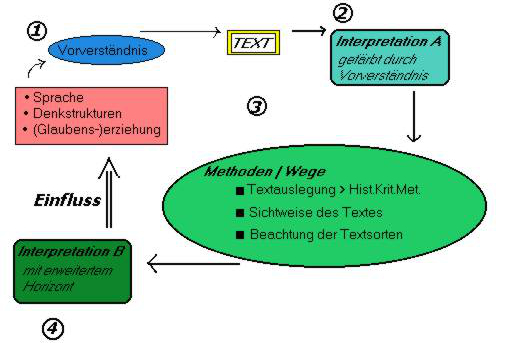
\includegraphics[width=0.8\linewidth]{Hermeneutik}
        \caption{Schematisches Schaubild des hermeneutischen Zirkels}\label{Hermeneutik}
    \end{center}
\end{figure}
\\Des weiteren muss man beachten, dass die Bibel im Original in Hebräisch und Altgriechisch geschrieben wurde. Die Bibel wurde also mehrmals übersetzt. So können mehrere Worte übersetzt das gleiche deutsche Wort ergeben, aber eine völlig unterschiedliche Bedeutung haben. Auch wenn die meisten nicht die Bibel in der Originalsprache lesen können, so muss man dies im Hinterkopf behalten, vor allem bei einzelnen kritischen Worten wie ``Hölle''. Ein Fehler, den man machen kann wie im dritten Reich, ist es, die Bibelstellen einzeln zu betrachten und nicht als ganzes in der Bibel. Mit einzelnen Stellen sind Fehlinterpretationen wahrscheinlicher und es können so martialische, ``antichristliche'' Ereignisse legitimiert werden wie die absolutistische Herrschaft von Adolf Hitler. Die effektivste Möglichkeit wäre theoretisch, für jeden Sachverhalt die Bibel von Anfang bis zum Ende zu untersuchen.
Zuletzt kann man die gegeben Stelle metaphorisch oder symbolisch betrachten, da Jesus und Gott mithilfe von Gleichnissen und Metaphern arbeiten. Diese Stellen sind meistens aber -zum Glück- leicht herauszufinden und zu deuten.
\begin{figure}[h]
    \begin{center}
        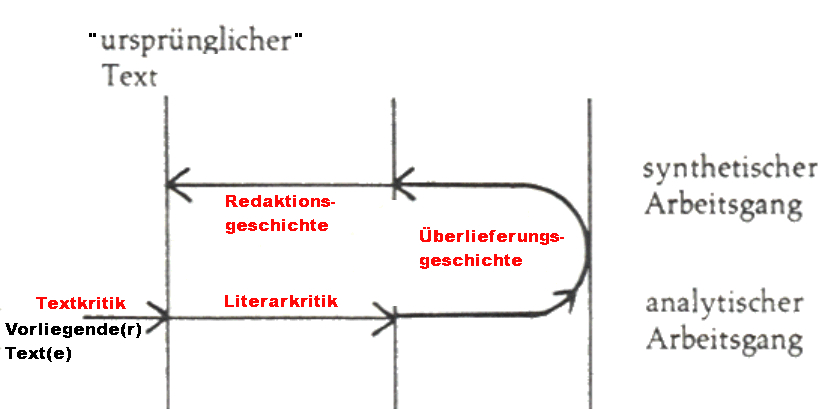
\includegraphics[width=\linewidth]{Historisch_kritische_Methode}
        \caption{Vereinfachtes Schaubild der historisch-kritischen Exegese}\label{HiKrMe}
    \end{center}
\end{figure}
\\Wie muss man also die Bibel verstehen? Es gibt keine Generallösung. Die eine Bibelstellen kann man direkt deuten, die anderen mithilfe von geschichtlichen Wissen, die andere mithilfe von verschiedenen Übersetzungen und die anderen metaphorisch. Und dann gibt es Stellen, die man auf alle Arten und Weisen deuten kann. Deshalb gibt es verschiedene Methoden wie die historisch-kritische Exegese (siehe Abb.\ \ref{HiKrMe}) oder den hermeneutischen Zirkel. Das einzige, was immer zutrifft, ist, dass man die Bibel immer als ganzes betrachten muss. Wann man wie was verstehen muss, muss man im jeden Fall einzeln abwägen. Dies macht das Bibelverstehen auch so schwierig und kontrovers. Zum Glück, jedoch nicht in allen Fällen und unter allen Umständen. Leider.



\chapter{Fazit}
Wichtig zu erwähnen ist, dass vieles hier auf Spekulationen, Hypothesen und Theorien beruht. Es gibt zwar Sachverhalte, die fundiert darzustellen sind, aber vieles fußt auf unbewiesenes und ist sogar heutzutage umstritten. Zweifelsfrei fließt neben der Wissenschaft auch sehr viel Glauben in dieses Fazit. Aber als ganzes bilden sie einen plausiblen Beweis, der nahezu alle meine Zweifel beseitigen kann.
\\
Die Bibel ist einzigartig. Sie ist zweifellos historisch Zuverlässig und es werden immer mehr archäologischen Funde bekannt, die dies immer mehr stützen. Die Bibel wurde nicht gravierend über die Zeit verfälscht und die Bibel, wie wir sie heute vorliegen haben, unterscheidet sich kaum von der damaligen Urfassung. Als Geschichtsschreibung und Geschichtswerk ist sie tadellos. Wenn man die Bibel anzweifelt, dann zweifelt man die Geschichte seit dem Mittelalter an und die gesamte Geschichtsschreibung.
\\~\\
Das Alte Testament ist von Gott inspiriert. In Anbetracht dessen, dass viele Menschen Gottes nahezu deckungsgleich schreiben, beweist dies nahezu. Die einzige Ausnahme sind die Vorschriften, Bräuche und Gesetzte der Priester oder anderer Machthaber und deren Legitimität. Diese wurden (bewusst oder unbewusst) durch die ``Machtgeilheit'' der Priester beeinflusst und sind so kritisch zu betrachten. Diese spielen aber zum Glück für das Christentum kaum eine Rolle und wurden im neuen Testament reformiert. Selbst die fragwürdigen Prophetien sind immer eingetreten und -wenn auch nur historisch gesehen- überliefert. Einzig in die Regel- und Ritualgebung sind menschliche Einflüsse zu verzeichnen, welche jedoch durch Jesus reformiert wurden.
\\~\\
Das Neue Testament ist auch von Gott inspiriert. Die Untersuchung der Autoren lässt darauf schließen, dass alle treue Nachfolger von Jesus und Gott waren. Widersprüche sind kaum zu finden und haben keinen großen Einfluss auf die Auslegung. Viele berichten indirekt oder direkt aus den Überlieferungen von Augenzeugen. Bei allen lassen sich -wenn auch nur hypothetisch- Motivationen nachweisen, welche auf eine göttliche Inspiration fußen und bei allen war der Zweck der Schrift einzig und allein die Verbreiten der Lehren Jesu und zwar so, wie er sie gelehrt hat oder wie er sie auslegen würde. Einzig die Offenbarung des Johannes muss kritisch angesehen werden. Zwar wurden die früheren Propheten des Alten Testaments als von Gott inspiriert eingestuft, jedoch ist bei diesen die Prophetie eingetreten, was bei der Offenbarung nicht behauptet werden kann. Erst wenn wir uns in der Endzeit und der Apokalypse befinden, können wir sicher sein, dass die Offenbarung göttlich inspiriert ist.
\\~\\
Gestützt durch Wissenschaft, plausiblen Theorien und Glauben kann ich reines Gewissens sagen: Die Bibel als Ganzes ist die heilige Schrift. Sie ist das Wort Gottes.
\chapter{Anmerkungen}
\section{Bibelkritik ist erlaubt}
Die Bibel wird unter Fachkreisen als Gotteswort in Menschenwort bezeichnet. Gotteswort, weil der Inhalt vom heiligen Geist gegeben wurden und Menschenwort, da der Verfasser diese empfangen, auslegen und verbreiten musste. Gottes Wort ist unfehlbar, aber wie die Fehlbarkeit des Menschen ist das Menschenwort selber fehlbar. Der simple Sachverhalt, dass Gottes Wort erst von einen Menschen empfangen, mit dessen Verstand ausgelegt, interpretiert, verfasst und einer teilweise langen Redaktion durchlaufen muss, erhöht die Wahrscheinlichkeit für Fehler. Deshalb ist Bibelkritik durchaus erlaubt, da das Menschenwort fehlbar ist und Gotteswort -im Gegensatz z.B. zum Koran- nicht wortwörtlich diktiert wurde.
\\~\\
Dies sieht man auch sehr gut in den Konflikten innerhalb der Bibel. Mose predigte noch, dass Juden keine nicht-jüdische Ehepartner haben dürfen. Bei einen Verstoß müssten diese und die zwei folgenden Generationen aus der jüdischen Gemeinde ausgeschlossen werden. David hatte nicht-jüdische Großeltern und war nebenbei noch der König des damaligen Israels. Von der Ausschluss aus der Gemeinde fehlt jede Spur. Das Alte Testament entstand in  1000 Jahren und das merkt man ihm an. Dies hat nicht zur Konsequenz, dass die ganze Bibel eine Lüge ist, vielmehr ist es eine Aufforderung, die Bibel kritisch zu lesen, aber auch selbstkritisch. Die Bibel ist Gottes lebendiges Wort, sodass die 3000 Jahre alten Worte noch heute Aktualität haben und neu ausgelegt werden müssen. Deshalb müssen wir die Bibel selbstkritisch lesen, sodass das lebendige Wort Gottes auch unser leben verändern kann und nicht zu einen toten Wort wird.

\section{Definition von Inspiration}
Während dieser Untersuchung wurde zu häuft von der göttlichen Inspiration geredet. Der Begriff ist ziemlich selbsterklärend. Die göttliche Inspiration meint, ob ein Autor wirklich sein Wissen durch und mit den heiligen Geist niedergeschrieben hat oder ob alles  lediglich seiner Fantasie entspringt. Doch letztendlich kann der Begriff doch nicht so einfach behandelt werden, wie er es anmuten lässt.
\\~\\
Welche Person als wirklich inspiriert zu betrachten ist und wodurch sich die göttliche Inspiration auszeichnen lässt ist eine sehr umstrittene Kernfrage der Bibelwissenschaften. Unterschieden wir in vielerlei Hinsicht. Es gibt die Modelle der Personen-, der Real- und der Ganzinspiration und alle bergen sie den Anspruch, die Inspiration eines Verfassers wissenschaftlich belegen zu können. Doch schlussendlich treffen sie auf dasselbe Problem: Eine solche Inspiration kann man nicht beweisen, da man sich in einen Bereich befindet, der sich außerhalb der empirisch erfassbaren Größen der Wissenschaft bewegt und so nicht eindeutig bewiesen werden kann.
\\~\\
Es kann nur unter personenspezifischen Grundannahmen beurteilt werden, d.h.\ man erachtet eine Person als göttlich inspiriert und leitet daraus die Charakteristika  einer solchen Inspiration ab, die man dann weiter übertragen kann. Hat man diese auf eine anderen Verfasser übertragen und erachtet ihn so auch als göttlich inspiriert, kann man wiederum aus seiner Schrift Charakteristika ableiten und weiter übertragen. Daraus entsteht dann ein Modell, welches unter bestimmten Grundannahmen beruht. Die Grundannahme bestimmt das ganze Modell. Das Glück des Christentum ist, dass alle an Jesus Christus als Sohn Gottes glauben und z.B. an Paulus als der erste große Theologe des Christentums, den Christus selbst begegnet ist. Somit sind einheitlich anerkannte Autoritäten vorhanden, aus denen man eigener maßen allgemein anerkannte Grundannahmen ableiten kann. Ohne solcher glücklichen Sachverhalte würden sich Modelle in noch größeren Dimensionen unterscheiden.
\\~\\
Des weiteren spielt das Bibelverständnis eine Rolle. Ein Fundamentalist wird kaum die göttliche Inspiration anzweifeln. Ein Historisch-kritischer Theologe jedoch schon. Der eine sieht die Bibel als Gottgegebenes Wort, der andere als eine Schrift von vielen Schriften. In dieser Arbeit wird die Bibel als Zeugenberichte verschiedener Personen betrachtet, die ihre Erfahrungen, Erlebnisse oder Offenbarungen niedergeschrieben haben. So ist jedes Buch nicht mehr als ein Zeugnis. Die Ausnahme bilden die Evangelien. Dies ist auch ein Bericht von einen Zeugen. Jedoch ist es ein Zeugnis von den Taten und Lehren Jesus. Wer nicht an der Glaubwürdigkeit der Evangelien zweifelt und Jesus als Gottes Menschwerdung sieht, für den hat der Inhalt einen absoluten Wahrheitsanspruch.
\\~\\
Aus diesen Gruüden wurde auf ein komplexeres Modell verzichtet. Die göttliche Inspiration wurde jeweils von der Motivation, dem Glaubensleben und den persönlichen Hintergrund abgeleitet. Letztendlich ist die Frage nach der göttlichen Inspiration eine Glaubensfrage, die sich jeder selber mit Ja oder Nein beantworten muss, unabhängig von den Modellen dritter, die aus deren Präferenzen und Vorstellungen entsprungen sind. Manchmal muss man sich aus seinen komplexen Denken und Ansprüchen raus lösen und auf einfache Fragen und Methodiken zurückbesinnen. Die Frage nach der göttlichen Inspiration ist eine und daher wurden hier nur zwei simple Fragen gestellt: Können Beruf, Motivation und Berufung auf eine göttliche Inspiration hindeuten? und/oder Kann ich den Verfasser genug vertrauen, um seine Schrift als göttlich Inspiriert zu betrachten?

\section{Kanonisierung}
Da der Zweck dieser Überprüfung ist, zu schauen, ob die heutige Bibel glaubwürdig ist und nicht, ob die Bibel in heutiger Form anders aussieht, als sie aussehen sollte, wurde der Aspekt der Kanonisierung nicht explizit angesprochen, obwohl es eine wichtige Rolle in dem Entstehungsprozess der Bibel spielt. Daher gibt es nur ein paar Anmerkungen zur Kanonisierung.
\\~\\
Es gab fünf Richtlinien, nach denen entschieden wurde, ob einen Schrift kanonisch, also zu heiligen Schrift gehörig, sein soll.
\\
1. Ist es autoritativ? --- Kam es von der Hand Gottes?
\\
2. Ist es prophetisch? --- War es von einen Mann Gottes geschrieben?
\\
3. Ist es authentisch? --- Es galt die Einstellung, bei Zweifel diese Frage zu verneinen, um so die Gültigkeit der Beurteilung der kanonischen Bücher sicherstellen zu können.
\\
4. Ist es dynamisch? --- Besaß es die lebenserneuernde Kraft Gottes?
\\
5. Wurde es angenommen, gesammelt, gelesen und gebraucht? Wurde es vom gläubigen Gottesvolk akzeptiert?
\\
Es ist offensichtlich, dass diese Gesichtspunkte sicherstellen sollten, dass eine Schrift göttlich inspiriert und kein Hirngespinste waren bzw.\ sind. Es ist also auch als eine Art Fragenkatalog zur göttlichen Inspiration zu sehen, der um einen kirchenpolitischen Gesichtspunkt (Siehe 5.) erweitert wurde.
\\~\\
Die Kanonisierung des Alten und des neuen Testaments ist ein langwieriger Prozess gewesen, dessen Betrachtung den Rahmen sprengen würde. Wichtig zu wissen ist, dass es bereits eine Entwicklung des Kanons vor den offiziellen Konzilen gab, in dem der Kanon in ähnlicher Form wie heute existierte. Der Vorwurf, dass ein Paar kirchenpolitische Entscheidungsträger willkürlich entschieden hätten, welche Schrift kanonisch ist oder nicht ist unangebracht.
Zudem haben sich genügend kluge Menschen und Denker darüber die Köpfe zerbrochen, welche Schrift denn nun kanonisch sei und welche nicht, sodass man diesen Kanon durch die große Masse an Debatten annehmen kann.